\chapter[Results]{Results}
\label{cha:Results}

This chapter shows the results that could be obtained through the experiments, mentioned in chapter \ref{cha:Experiment}. Those results contain either numbers, for assessing the model performance with a certain error performance, but also of graphics, displaying the outputs of the models. The outputs of the models, being spectrograms, are compared with their corresponding input spectrograms. As the output of the encoder part (embedding) plays a crucial role regarding audio synthesis, those also get displayed and assessed further on. Some additional graphics containing additional spectrograms, embeddings and signal plots can be found in the appendix \ref{app:addional_graphics}. Regarding the final listenable sounds, those get discussed in the next chapter.

\section{Results regarding model with single frequency vectors}
As described in chapter \ref{cha:Experiment} experiments have been conducted by using the single frequency vectors of the spectrograms. As a model, a 18 layer deep neural network with 1D convolutions has been trained on the reconstruction of single frequency vectors. 
Throughout the development different settings have been tried out in order to find a model with an optimal training process and performance. The amount of data on which the model has been trained on, has been varied as different performances regarding the convergence could be observed. First trainings have been made on \texttt{keyboard\_synthetic} mixed with \texttt{guitar\_acoustic}. As a note, those two terms are labels from the dataset representing the instrument family and source. Here it could be observed that no sufficient convergence could be reached (MSE > 200). Training a distinct model per instrument source showed that the instrument source has a significant influence on the convergence. For example a model trained solely on \texttt{keyboard\_synthetic} converged better then a model with \texttt{guitar\_acoustic}. Comparing the performance of a network trained on \texttt{guitar\_acoustic} with one trained on e.g. \texttt{guitar\_electronic}, showed that with the latter a better score could be reached (\textasciitilde 17). Therefore the decision was made to combine \texttt{keyboard\_synthetic} and \texttt{guitar\_electronic} instead of acoustic, for the training. Compared to the one mixed with \texttt{guitar\_acoustic} a score of \textasciitilde 78 could be reached. Subsequently more instrument sources were added, until the whole training dataset was utilized. This model showed the best performance regarding its error scores and was chosen to be considered for the ongoing experiments. Table \ref{tab:res_scores_1Dcae} shows the error scores of this model. As a short note, each trained model was chosen based on the best validation error score. 

\begin{table}[htb!]
    \centering
    \begin{tabular}{|c|c|}
        \hline
         & \textbf{MSE-Score} \\
         \hline
        \textbf{Training} & 4,237 \\
        \hline
        \textbf{Validation} & 4,638 \\
        \hline
        \textbf{Test} & 1,190 \\
        \hline
    \end{tabular}
    \caption{MSE-Scores 1D convolutional autoencoder.}%\caption{MSE-Scores 1D convolutional autoencoder (8 epochs)}
    \label{tab:res_scores_1Dcae}
\end{table}

Here it can be seen that the error scores for training and validation are rather close, while the score on the held out test set was significantly smaller. This score could be reached with a training over 8 epochs and was considered as the best score, as after those 8 epochs the validation score increased again (despite decreasing training score). Table \ref{tab:res_scores_1D_pitch} is also interesting as it shows the error scores on the test set, regarding different pitches. As displaying all pitches would go beyond the scope, pitch classes from 030 to 100 have been chosen. In this case it can be seen that all error scores have roughly the same value and do not differ significantly. Nevertheless there is a small trend visible if the score increases depending the pitch.

\begin{table}[htb!]
    \centering
    \begin{tabular}{|c|c|}
        \hline
         \textbf{Pitch} & \textbf{MSE-Score} \\
         \hline
         \textbf{030} & 1,049\\
         \hline
         \textbf{035} & 1,393\\
         \hline
         \textbf{040} & 0,935\\
         \hline
         \textbf{045} & 1,096\\
         \hline
         \textbf{050} & 1,019\\
         \hline
         \textbf{055} & 1,108\\
         \hline
         \textbf{060} & 1,086\\
         \hline
         \textbf{065} & 1,111\\
         \hline
         \textbf{070} & 1,164\\
         \hline
         \textbf{075} & 1,041\\
         \hline
         \textbf{080} & 1,177\\
         \hline
         \textbf{085} & 1,753\\
         \hline
         \textbf{090} & 1,100\\
         \hline
         \textbf{095} & 1,796\\
         \hline
         \textbf{100} & 2,043\\
         \hline
    \end{tabular}
    \caption{MSE-Scores for specific pitch classes using 1D convolutional autoencoder.}
    \label{tab:res_scores_1D_pitch}
\end{table}

\subsection{Experiments of single reconstruction}
Having the trained network, this one got evaluated towards the ability of reconstructing audio spectrograms and further on recreating the sounds. The next graphics \ref{fig:res_1D_input_output}, \ref{fig:res_1D_emb} and \ref{fig:res_1D_input_output_sig} show the result of taking a guitar sample as input and reconstructing it. 

\begin{figure}[htb!]
    \centering
    \makebox[\textwidth][c]{\begin{tabular}{@{}cc@{}}
        \makebox{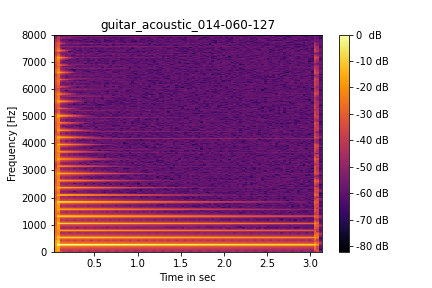
\includegraphics[width=0.50\textwidth]{images/approach/guitar_acoustic_014-060-127.png}}&
        \makebox{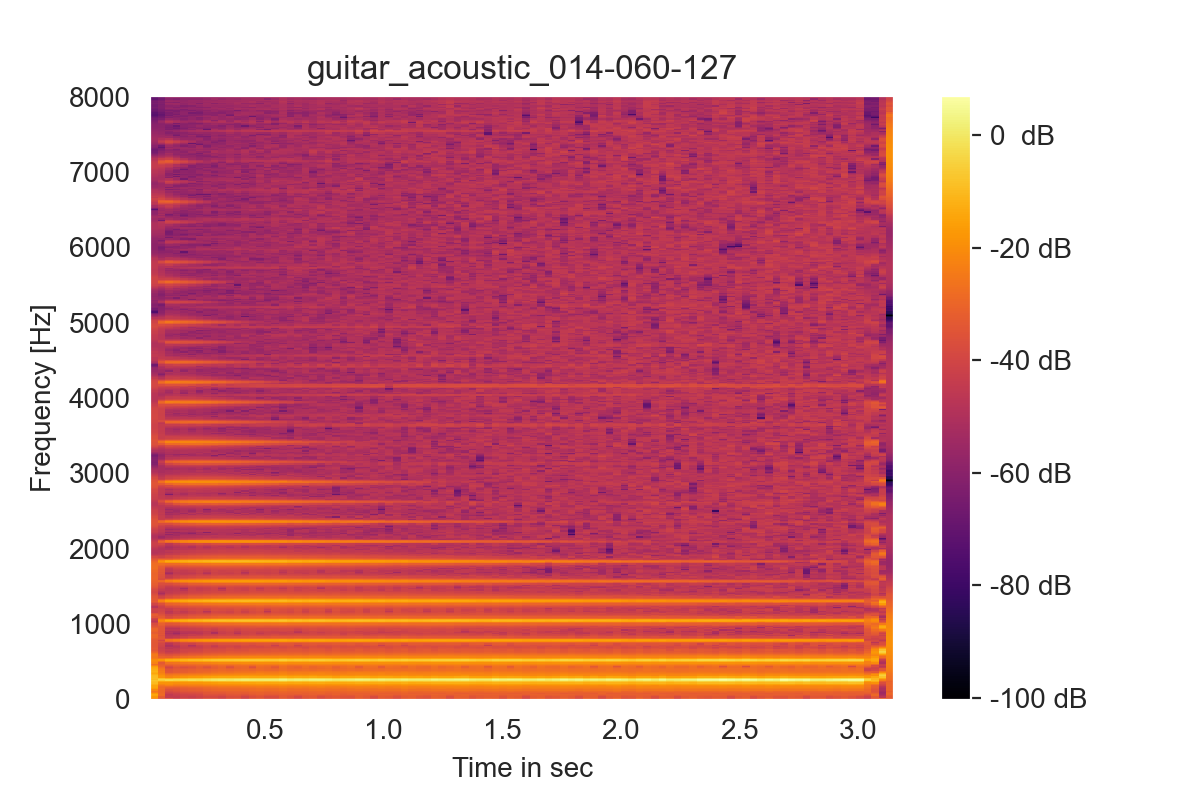
\includegraphics[width=0.50\textwidth]{images/results/rec_guitar_acoustic_014-060-127.png}}\\
        input spectrogram ~(a) & reconstructed spectrogram ~(b)
    \end{tabular}}
    \caption{Difference between input and reconstructed spectrogram.}
    \label{fig:res_1D_input_output}
\end{figure}

With a special look onto the reconstructability of spectrograms, figure \ref{fig:res_1D_input_output} shows the input spectrogram and the generated output spectrograms from the network. Here it can be seen that the reconstructed spectrogram differs in a few points from the input spectrogram. First of all it can be seen, that across the frequency areas that contain little energy in the input spectrogram, in the output more energy is present. This also means that between those areas and the sound-characteristic high energy areas, less difference is present. Furthermore regarding the original broad spectra at the beginning and at the end, those are hardly present in the output spectrogram. Knowing that these represent the stroke and the damp of the string, it can be said that these are not present in the output. This is also confirmed through looking at the time-domain signal.

\begin{figure}[htb!]
    \centering
    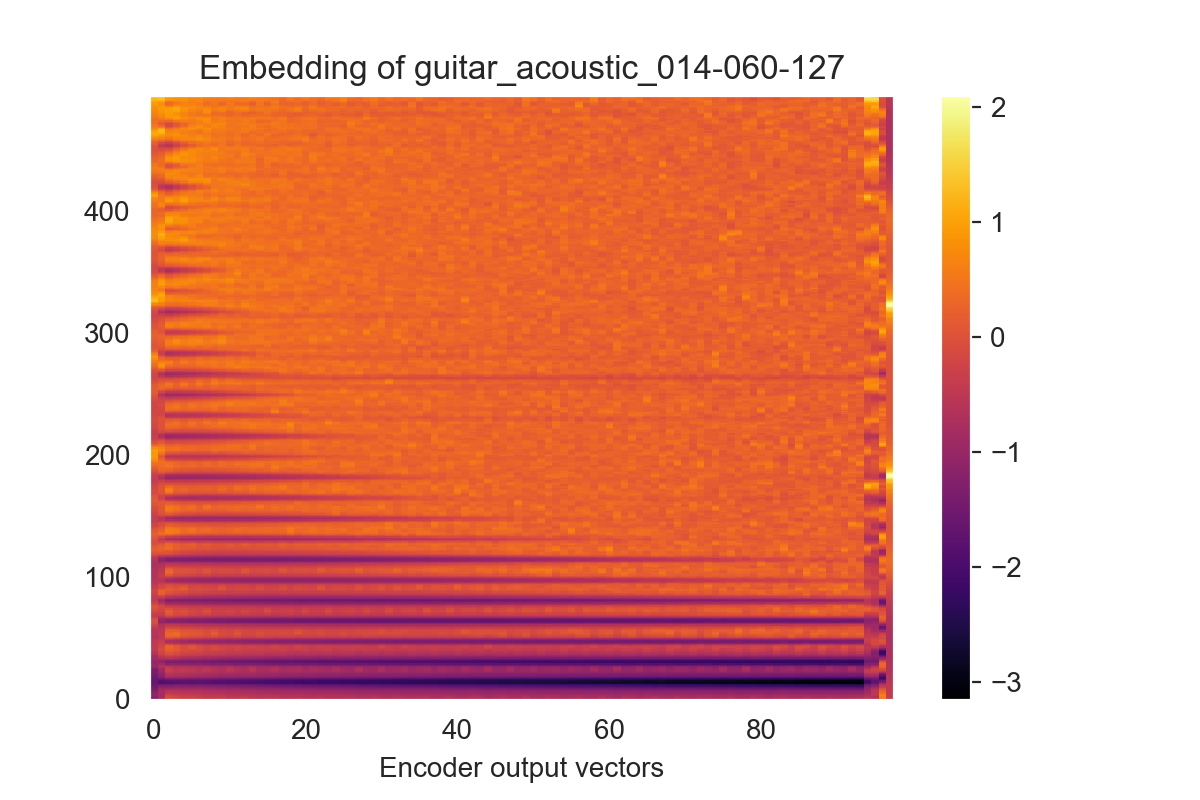
\includegraphics[width=0.60\textwidth]{images/results/emb_guitar_acoustic_014-060-127.png}
    \caption{Embedding of guitar acoustic.}
    \label{fig:res_1D_emb}
\end{figure}

Looking at the graphic that depicts the embedded space, there it already can be seen that those broad spectra are not preserved. Despite of that the high energy areas (harmonics) in the input spectrogram are preserved as negative values in the embedding while the original low energy areas get represented by positive values. Also as there are no strides applied in the network, there is almost no compression in the embedding.

A final look onto the time domain plots in figure \ref{fig:res_1D_input_output_sig} also reveal, that there's no impulse at the beginning of the signal. Furthermore it also can be said that the amplitude in general differs in its course but also in how strong it is.

\begin{figure}[htb!]
    \centering
    \makebox[\textwidth][c]{\begin{tabular}{@{}cc@{}}
        \makebox{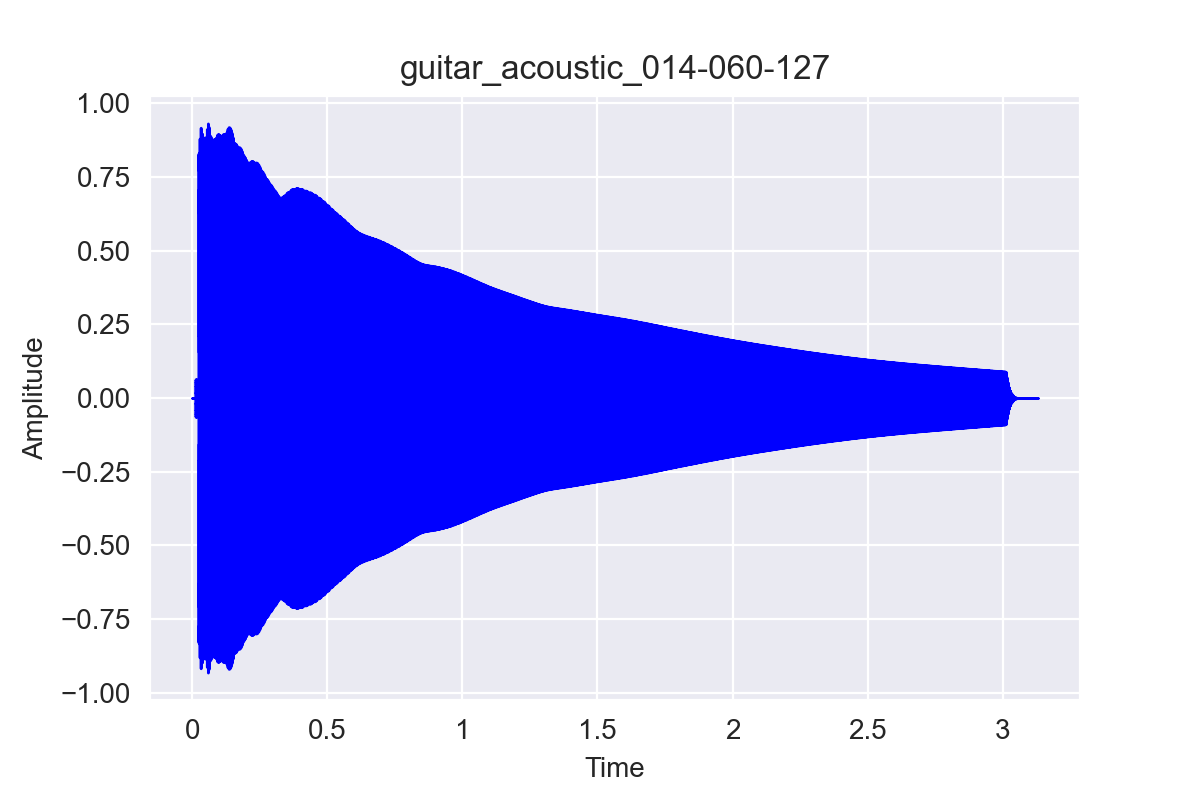
\includegraphics[width=0.50\textwidth]{images/results/inp_guitar_acoustic_014-060-127.png}}&
        \makebox{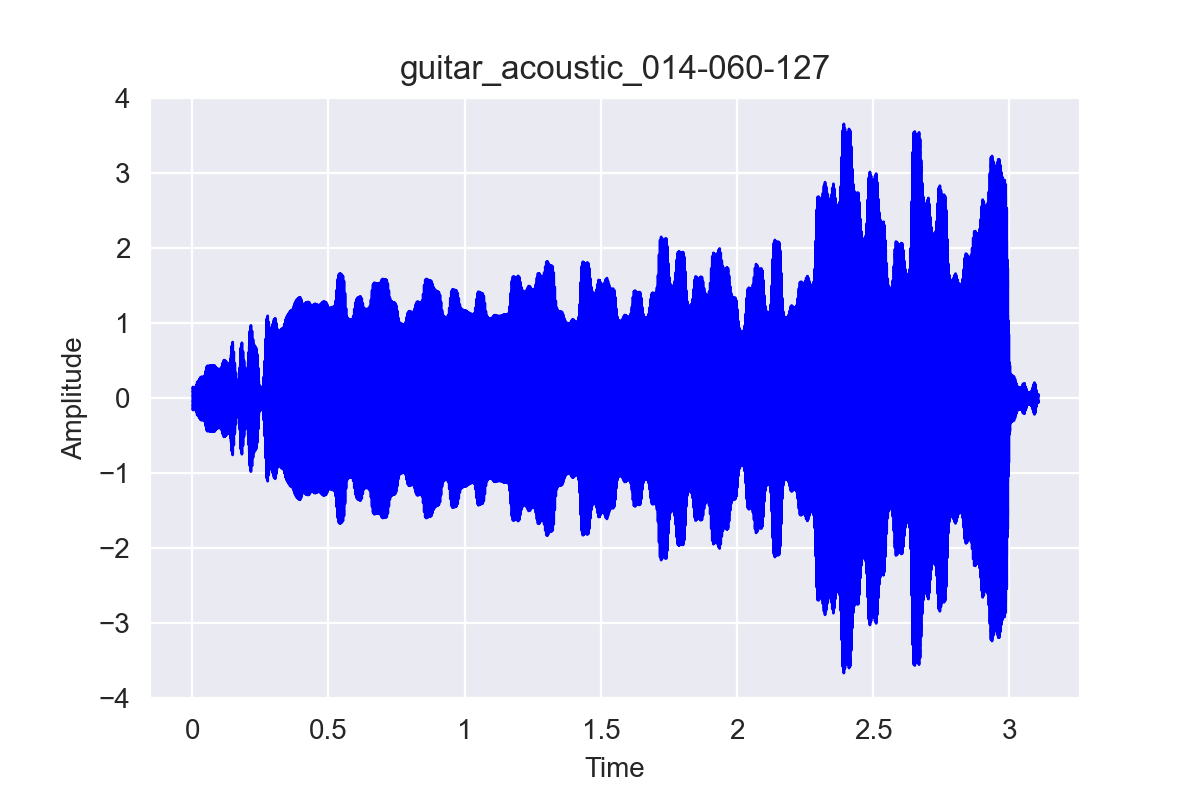
\includegraphics[width=0.50\textwidth]{images/results/out_guitar_acoustic_014-060-127.png}}\\
        input signal. ~(a) & output signal. ~(b)
    \end{tabular}}
    \caption{Differences between output and reconstructed time signal.}
    \label{fig:res_1D_input_output_sig}
\end{figure}


\subsection{Experiments with interpolation in embedding}
With this kind of 1D convolutional autoencoder first experiments were made, that use interpolation in embedded space to synthesize novel sounds. In chapter \ref{cha:Approach} and \ref{cha:Experiment} the concept has already been described in detail. Having this concept, instrument sources were chosen, which in order got encoded and interpolated together in order to form a new embedding. Figure \ref{fig:res_1D_input_interpolation} shows the spectrograms of the two input instruments that were chosen to create a novel sound. For this representation an acoustic guitar and acoustic brass sample were taken and encoded. By comparing those two spectrograms, it can be seen that they differ significantly in their structure. While it can be seen that the guitar looses energy in its higher frequency ranges, the brass sample keeps its frequency energy over the whole time. Furthermore as the harmonics stay constant in the guitar sample, those alternate in the brass. Those properties make it interesting to use them for the interpolation and thus synthesise a novel sound. For comparative reasons, in further experiments also those two instruments have been used for the synthesis task which can be seen later on.

\begin{figure}[htb!]
    \centering
    \makebox[\textwidth][c]{\begin{tabular}{@{}cc@{}}
        \makebox{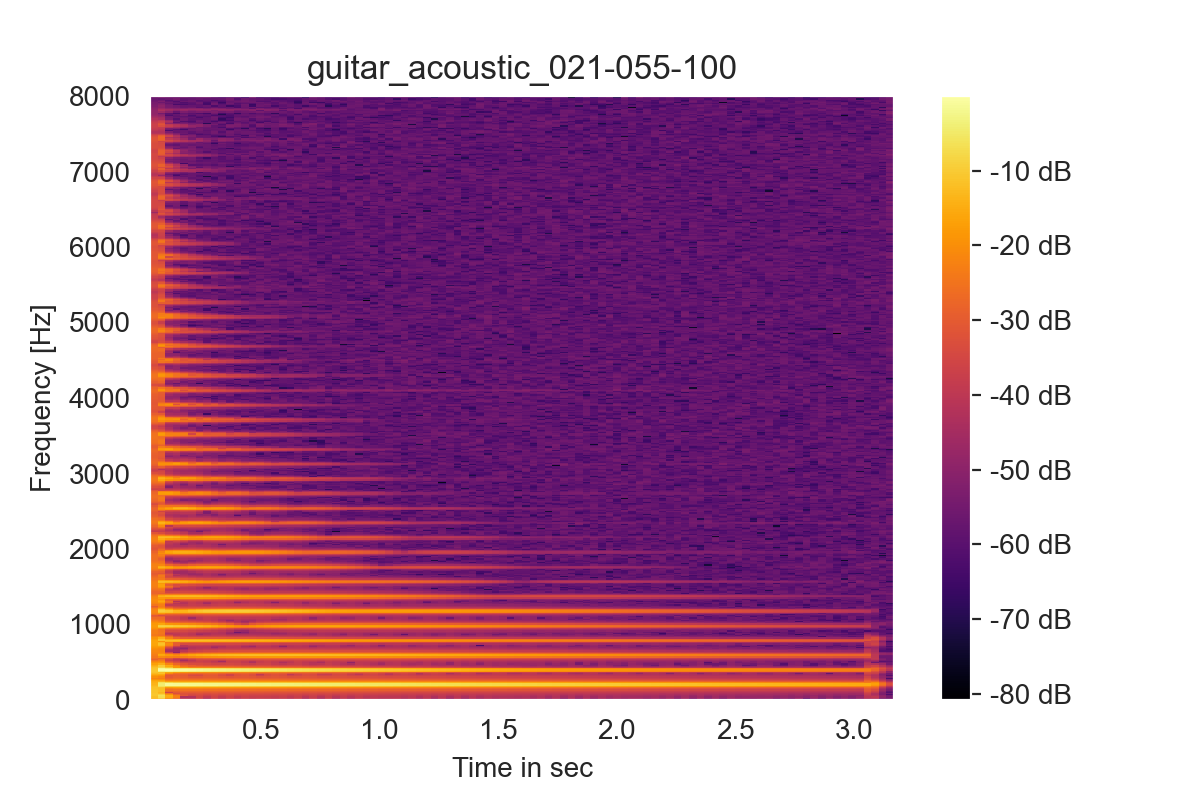
\includegraphics[width=0.50\textwidth]{images/results/guitar_acoustic_021-055-100.png}}&
        \makebox{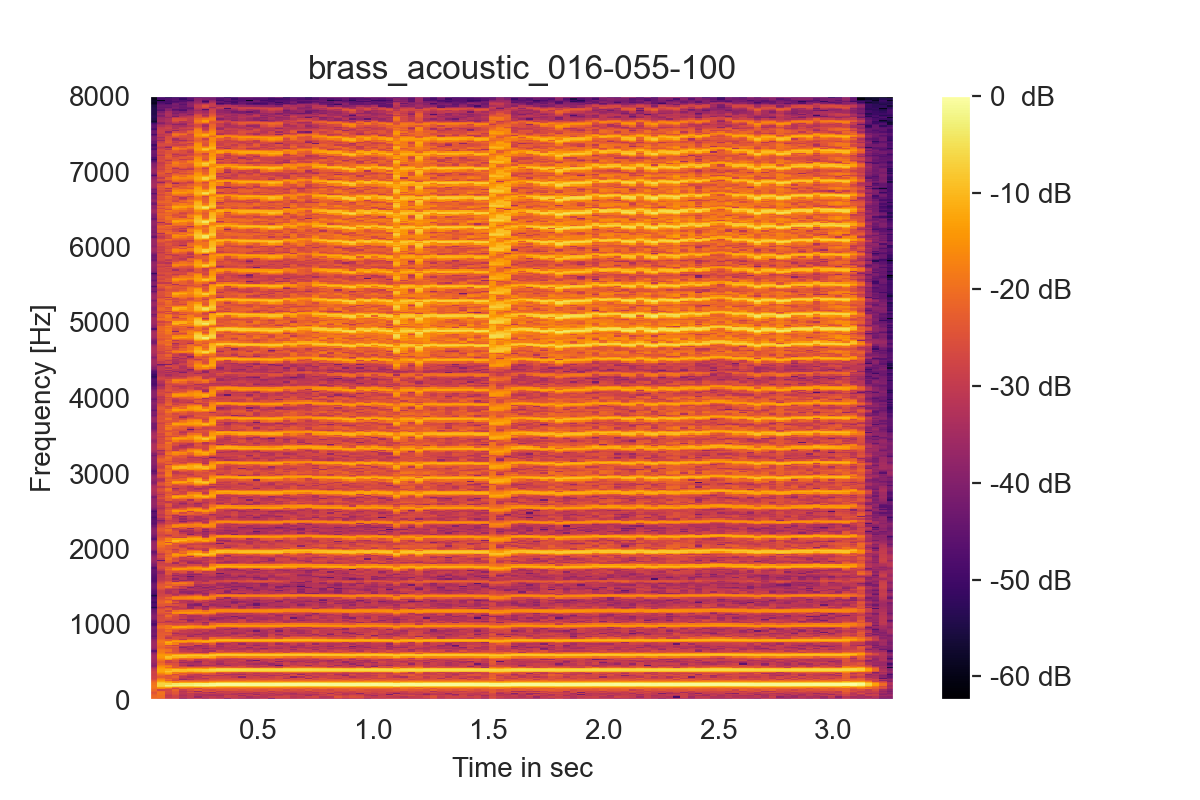
\includegraphics[width=0.50\textwidth]{images/results/brass_acoustic_016-055-100.png}}\\
        guitar acoustic ~(a) & brass acoustic ~(b)
    \end{tabular}}
    \caption{Input spectrograms.}
    \label{fig:res_1D_input_interpolation}
\end{figure}

After encoding, the outputs were taken and interpolated as can be seen in figure \ref{fig:res_1D_interpolation}a. As it can be seen, those embeddings are a compressed form of the input spectrograms. When looking onto the generated interpolated embedding, it can be said that this one incorporates both instruments encoded features. Having this new vector, this one was fed into the decoder network in order to generate an output spectrogram that can be seen in figure \ref{fig:res_1D_interpolation}b. 

\begin{figure}[htb!]
    \centering
    \captionsetup{justification=centering}
    \makebox[\textwidth][c]{\begin{tabular}{@{}c}
        \makebox{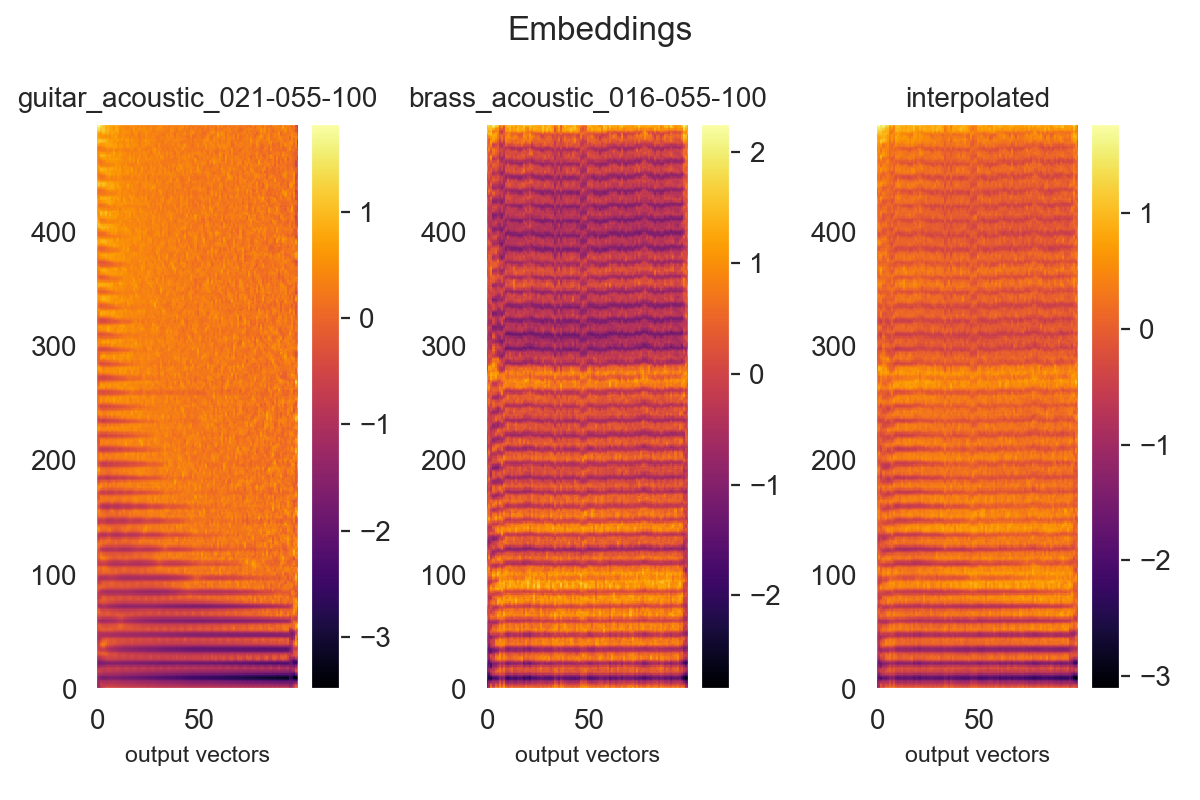
\includegraphics[width=0.60\textwidth]{images/results/interp_emb_guitar_acoustic_021-055-100&brass_acoustic_016-055-100.png}}\\
        embedding interpolation ~(a)\\
        \makebox{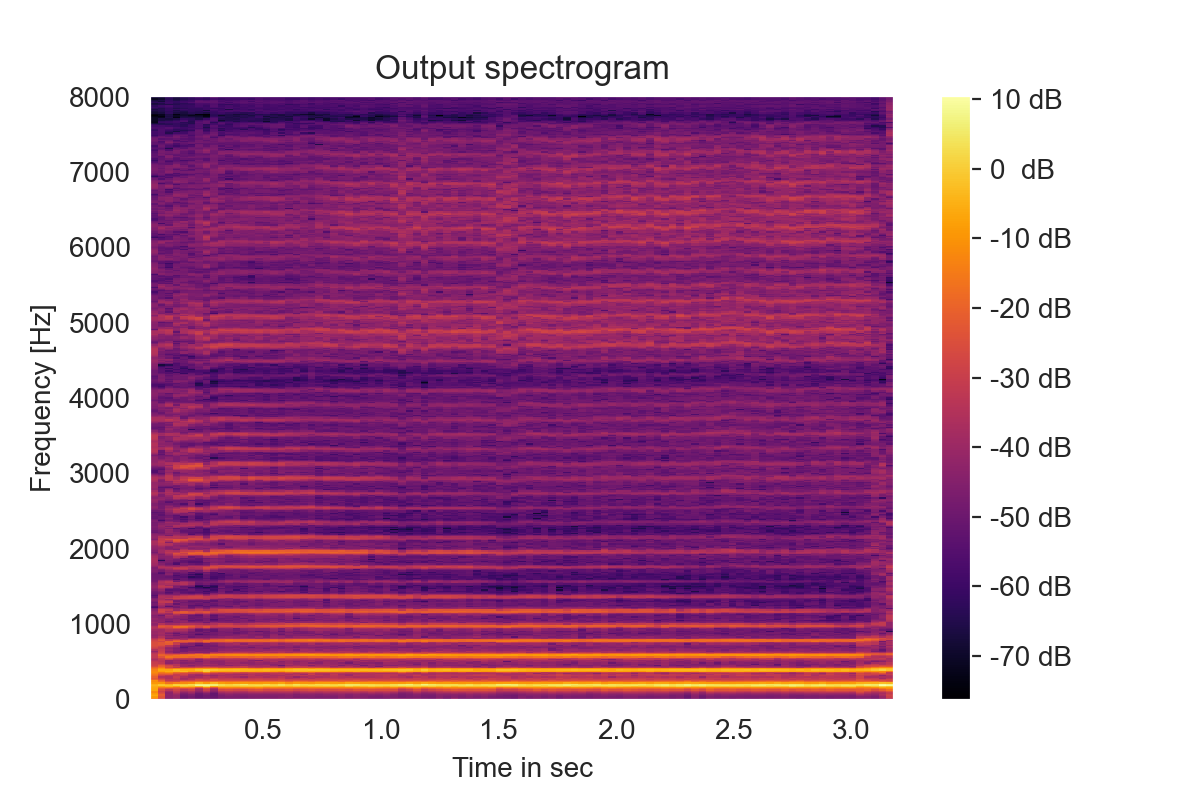
\includegraphics[width=0.60\textwidth]{images/results/guitar_acoustic_021-055-100&brass_acoustic_016-055-100_output_spec.png}}\\
        output signal ~(b)
    \end{tabular}}
    \caption{Embeddings of input samples with interpolated embedding and its corresponding output spectrogram.}
    \label{fig:res_1D_interpolation}
\end{figure}

Having the final spectrogram here as output, it can be seen that spectral data of both input spectrograms are basically contained. Similar to the output spectrogram in figure \ref{fig:res_1D_input_output}b this one also does not contain the impulse (guitar stroke) at the beginning. To finally obtain a listenable sound, the output spectrogram has to be converted back to time-domain, which in this case is done with the Griffin-Lim algorithm \cite{Griffin1984} as no phase information is present. To improve the quality of the output but also to examine the performance of other types of networks some further experiments have been made using 2D convolutions but also additional post-processing steps.

\section{Results of experiments with spectrogram frames}
The here shown results correspond to the described experiments in section \ref{sec:exp_spec_slice}. Here again a 2D convolutional autoencoder has been utilized to (re)synthesize audio. As input data for the neural networks, overlapping spectrograms snippets with the length of 3 along the time axis have been considered. In contrast to the previous network, this was supposed to bring better results, regarding the output but especially to preserve transients. As different networks with different stridings (compression) were trained and used, the results should also show the differences in the output but also in their quality regarding audio (re)synthesis. Additionally the encoded data gets examined by calculating the correlation coefficients between samples (mostly of the same pitch). By that it can be seen how much the encodings of different instruments differ. Additionally it also can be examined how good the different networks extract the essential features of the input data. Throughout the project these correlation coefficients got depicted in a so-called correlation matrix. Displaying one here would would not work out sufficiently, as because of its many values, those are hardly readable without zooming in. Because of this, just the findings are discussed later on in chapter \ref{cha:Discussion}. Finally also additional post-processing steps get applied, which help to correct the energy and thus the quality of the output. The results shown here are without energy correction, but the effect will also be discussed later on in the discussion.

The following table \ref{tab:res_scores_2Dcae} shows the MSE error scores of the different 2D convolutional networks. As mentioned in chapter \ref{cha:Experiment}, three networks were trained, that differ in their configuration regarding striding and thus have different embedding sizes. These networks therefore are called single, double- and triple stride networks, regarding the amount of striding on each network side. By this they can be distinguished better in this work. In table \ref{tab:res_scores_2Dcae} it can be seen that by using a different amount of strides, this has an impact on the score. The network with just one stride on each side has the lowest error whereas the networks with two or three strides have a significantly higher error. Regarding the difference between training, validation and testing error all three networks show the same behaviour as the validation error is higher than the training error with the test score being the best. 

\begin{table}[htb!]
    \centering
    \captionsetup{justification=centering}
    \begin{tabular}{|c|c|c|c|}
        \hline
         & \textbf{single-stride} & \textbf{double-stride} & \textbf{triple-stride} \\
         \hline
        \textbf{Training} & 9,779 & 13,717 & 18,292 \\
        \hline
        \textbf{Validation} & 10,094 & 14,056 & 19,056 \\
        \hline
        \textbf{Test} & 7,831 & 10,711 & 16,655 \\
        \hline
    \end{tabular}
    \caption{MSE-Scores 2D convolutional autoencoder - single stride, double stride, triple stride.}
    %\caption{MSE-Scores 2D convolutional autoencoder - single stride (9 epochs), double stride (8 epochs), triple stride (16 epochs).}
    \label{tab:res_scores_2Dcae}
\end{table}

Compared to the error score of the 1D convolutional network, it can be said that all error scores are significantly higher. In case of this work, the score does not mean that the quality of the output is worse, especially regarding the final output sound. The latter will be discussed later on in the discussion of this work.

As during the previous experiment also the scores regarding different pitches were calculated, the next table \ref{tab:res_scores_2D_pitch} shows the different scores regarding pitches ranging from 30 to 100. Similar to the 1D convolutional network, the error scores regarding the pitch do not show a specific trend. Interestingly the scores of the triple-strided network have some rather strong outliers regarding samples around the classes 045-050. Having the same error scores this also does not mean that all pitches have the same audible quality, but more on that in chapter \ref{cha:Discussion}. 


\begin{table}[htb!]
    \centering
    \begin{tabular}{|c|c|c|c|}
        \hline
         \textbf{Pitch} & \textbf{single-stride} & \textbf{double-stride} & \textbf{triple-stride}\\
         \hline
         \textbf{030} & 7,084 & 9,175 & 12,241\\
         \hline
         \textbf{035} & 7,912 & 12,294 & 15,426\\
         \hline
         \textbf{040} & 7,292 & 11,205 & 18,639\\
         \hline
         \textbf{045} & 7,251 & 12,434 & 22,151\\
         \hline
         \textbf{050} & 6,840 & 9,903 & 20,287\\
         \hline
         \textbf{055} & 7,535 & 10,434 & 18,102\\
         \hline
         \textbf{060} & 7,444 & 10,128 & 17,670\\
         \hline
         \textbf{065} & 8,313 & 10,286 & 16,497\\
         \hline
         \textbf{070} & 7,410 & 9,868 & 14,894\\
         \hline
         \textbf{075} & 7,850 & 9,949 & 14,273\\
         \hline
         \textbf{080} & 8,624 & 10,529 & 15,486\\
         \hline
         \textbf{085} & 9,299 & 11,090 & 16,598\\
         \hline
         \textbf{090} & 8,798 & 11,435 & 16,415\\
         \hline
         \textbf{095} & 9,948 & 12,032 & 17,049\\
         \hline
         \textbf{100} & 12,346 & 13,179 & 19,812\\
         \hline
    \end{tabular}
    \caption{MSE-Scores for specific pitch classes using 2D convolutional autoencoder.}
    \label{tab:res_scores_2D_pitch}
\end{table}

\subsection{Experiments of single reconstruction}
Having mentioned the error scores regarding reconstructing spectral audio data, those cannot be taken solely to assess the performance of the network. Therefore experiments, like with the previous network, were conducted in recreating single spectrograms. With those the ability towards reconstructing audio spectrograms becomes assessed visually and auditorily for the purpose of audio (re)synthesis.
For comparative reasons, the same spectrogram source has been chosen like with the previous network. As the original input spectrogram has already been shown in figure \ref{fig:res_1D_input_output}a, here just the output of the encoder part (embedding) but also the total output gets depicted (see figures \ref{fig:res_single_str_2D_output_emb}, \ref{fig:res_double_str_2D_output_emb} and \ref{fig:res_triple_str_2D_output_emb}). The spectrograms in each of these graphics were generated with single-, double- and triple-stride networks and do not contain the energy correcting post-processing mechanism. Despite of this fact, it can be seen when looking onto all the output spectrograms (\ref{fig:res_single_str_2D_output_emb}a, \ref{fig:res_double_str_2D_output_emb}a and \ref{fig:res_triple_str_2D_output_emb}a), that all preserve the broad spectra at the beginning and ending of the spectrograms, especially by looking onto the first one. When comparing again the low energy areas of the input spectrogram to the output spectrograms, it can be said that they also contain similarly little energy. Again it can also be seen that the embedding looks like a spectrogram but in a compressed form of the input, as it also contains similar structures. Contrary to the embedding in figure \ref{fig:res_1D_emb} the high energy areas have positive numbers while original low energy area have negative numbers.

\begin{figure}[htb!]
    \centering
    \captionsetup{justification=centering}
    \makebox[\textwidth][c]{\begin{tabular}{@{}cc@{}}
        \makebox{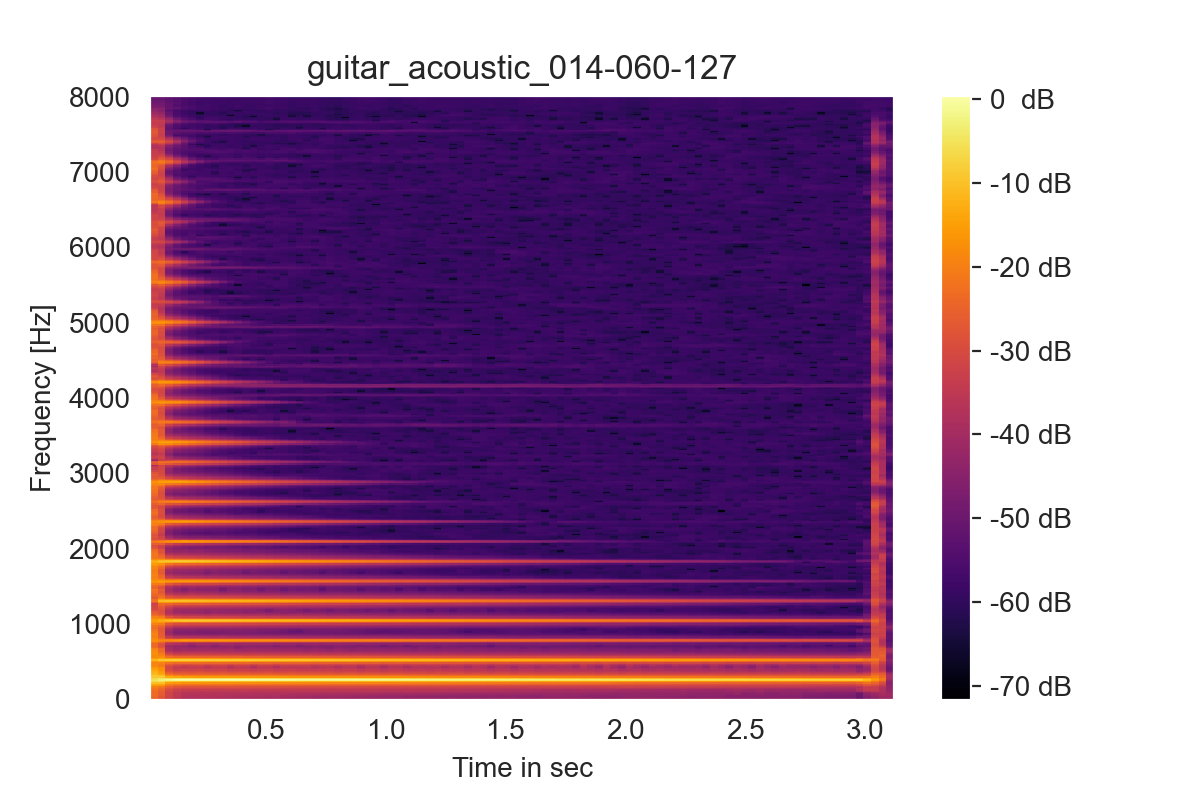
\includegraphics[width=0.50\textwidth]{images/results/single_str/out_guitar_acoustic_014-060-127.png}}&
        \makebox{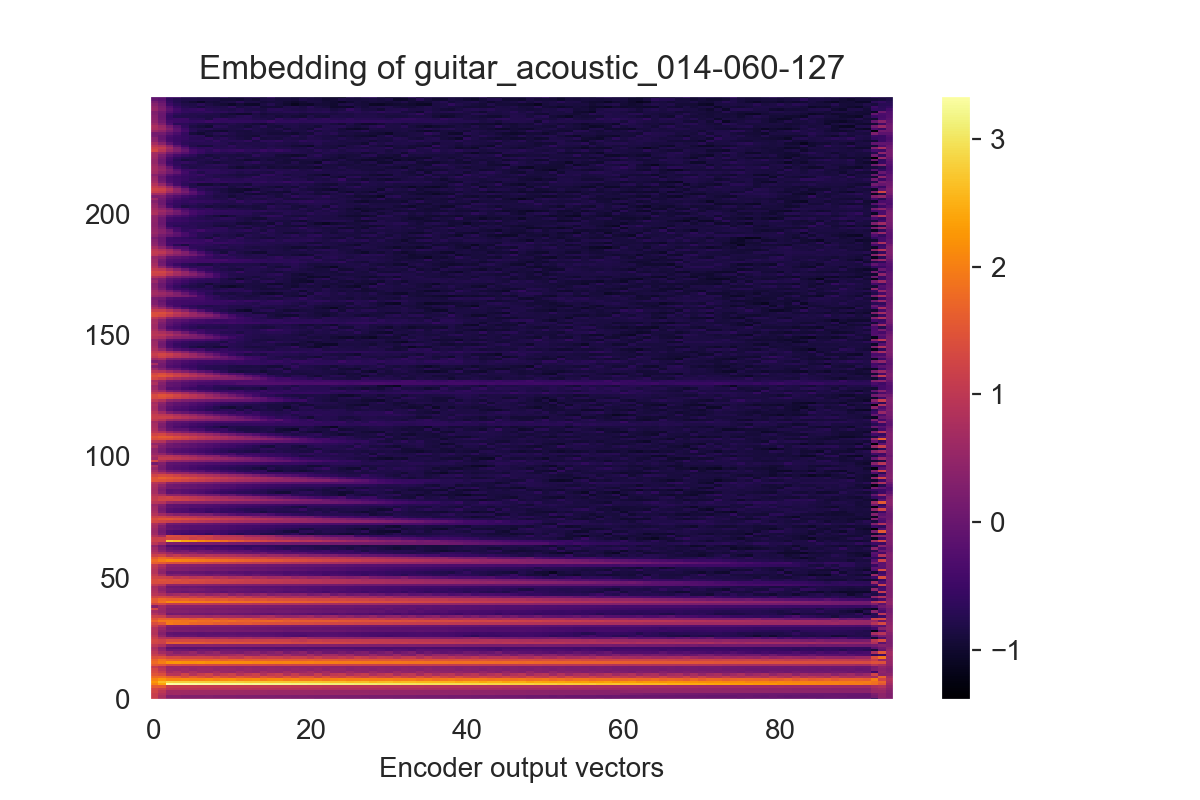
\includegraphics[width=0.50\textwidth]{images/results/single_str/emb_guitar_acoustic_014-060-127.png}}\\
        reconstruction of guitar acoustic ~(a) & embedding of guitar acoustic ~(b)
    \end{tabular}}
    \caption{Reconstructed spectrogram and corresponding embedding - single-stride model.}
    \label{fig:res_single_str_2D_output_emb}
\end{figure}

With a look on the output of the double-stride network (figure \ref{fig:res_double_str_2D_output_emb}a), it also can be said that the broad spectra are preserved but with less energy. This can be also noticed when looking on the output spectrogram of the triple stride network (figure \ref{fig:res_triple_str_2D_output_emb}). The latter also shows less energy in the high energy areas and less "precise harmonics" (washed out). 

\begin{figure}[htb!]
    \centering
    \captionsetup{justification=centering}
    \makebox[\textwidth][c]{\begin{tabular}{@{}cc@{}}
        \makebox{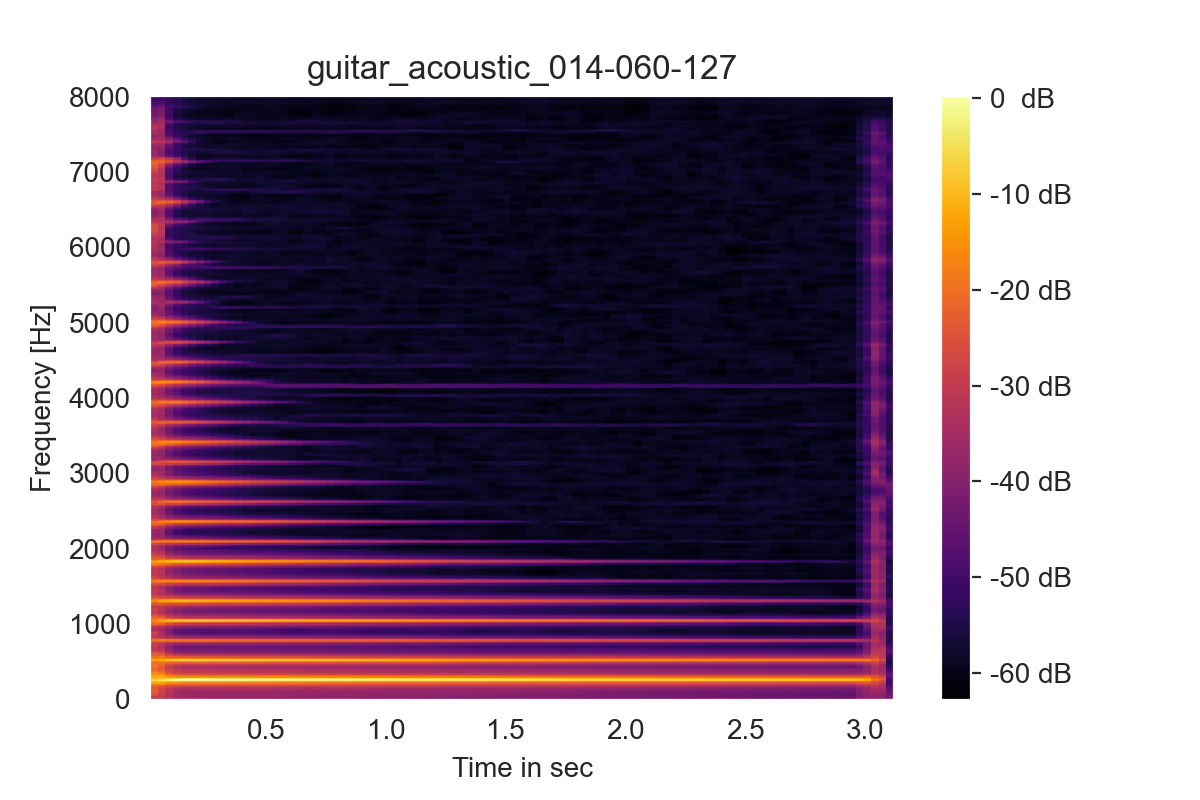
\includegraphics[width=0.50\textwidth]{images/results/double_str/guitar_acoustic_014-060-127.png}}&
        \makebox{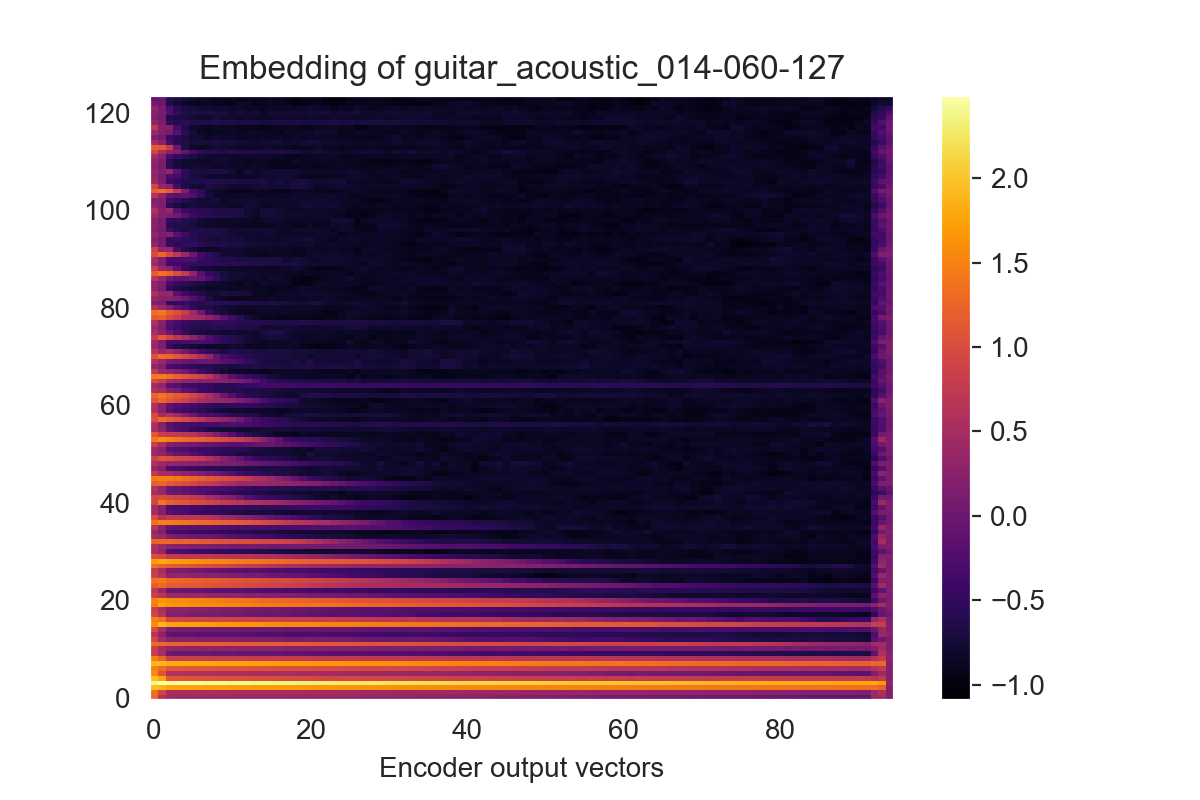
\includegraphics[width=0.50\textwidth]{images/results/double_str/emb_guitar_acoustic_014-060-127.png}}\\
        reconstruction of guitar acoustic ~(a) & embedding of guitar acoustic ~(b)
    \end{tabular}}
    \caption{Reconstructed spectrogram and corresponding embedding - double-stride model.}
    \label{fig:res_double_str_2D_output_emb}
\end{figure}

Looking onto the embeddings of the two networks it can be said, that those contain significantly less values across the y-axis. Comparing it to the input but also the output, despite of the significant compression, the significant harmonic features and general structures are present as positive numbers (regarding the colorscale). As concerning the double strided network, the embedding still has a fine granularity contrary to the one obtained by the triple strided network.

\begin{figure}[htb!]
    \centering
    \captionsetup{justification=centering}
    \makebox[\textwidth][c]{\begin{tabular}{@{}cc@{}}
        \makebox{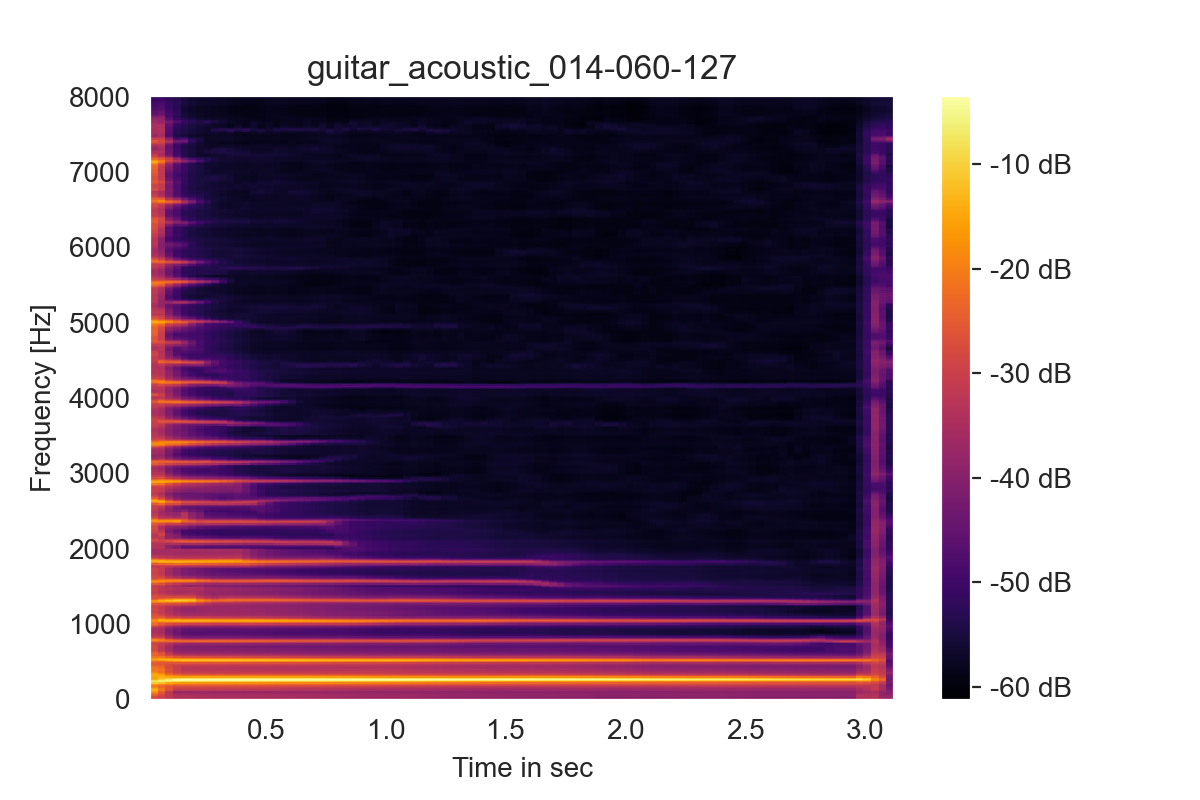
\includegraphics[width=0.50\textwidth]{images/results/triple_str/guitar_acoustic_014-060-127.png}}&
        \makebox{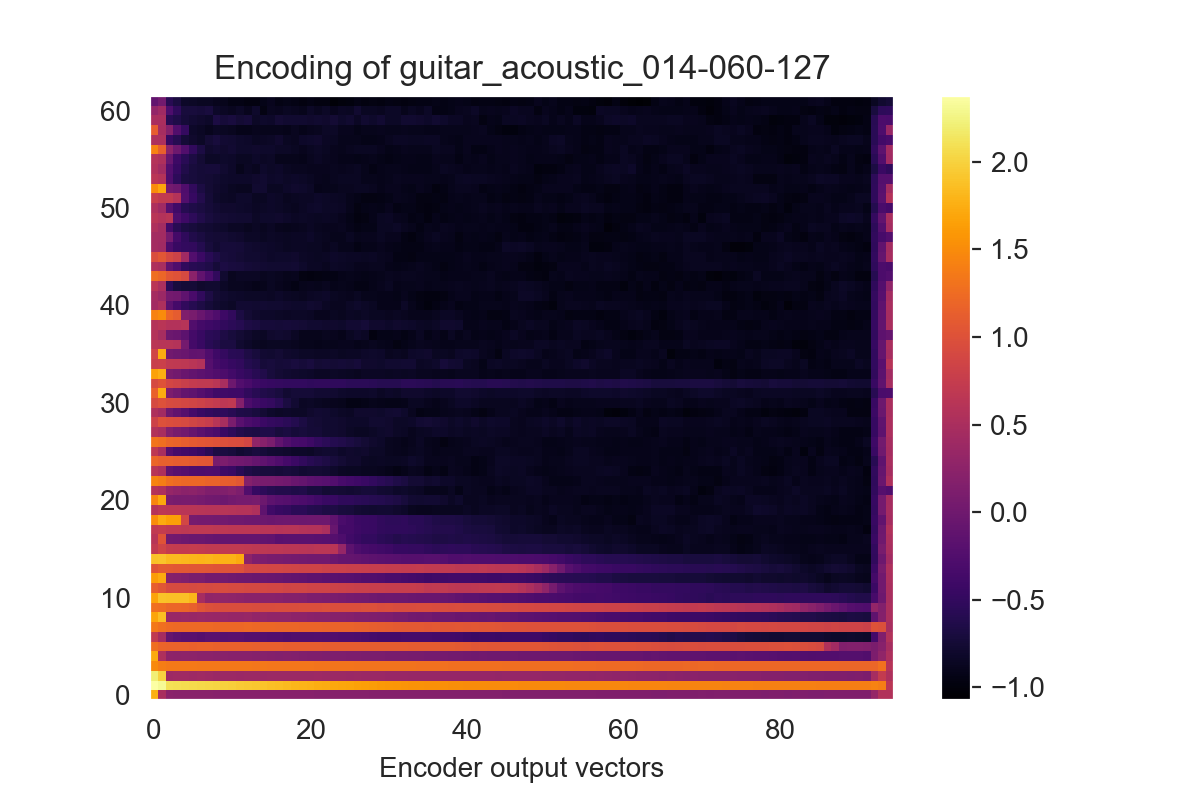
\includegraphics[width=0.50\textwidth]{images/results/triple_str/emb_guitar_acoustic_014-060-127.png}}\\
        reconstruction of guitar acoustic ~(a) & embedding of guitar acoustic ~(b)
    \end{tabular}}
    \caption{Reconstructed spectrogram and corresponding embedding - triple-stride model.}
    \label{fig:res_triple_str_2D_output_emb}
\end{figure}

\subsection{Experiments with interpolation in embedding}
The results in this section show the resulting output spectrograms that got generated by interpolation of the embedding space vectors. This has already been done with the 1D convolutional network where novel sounds could be generated. As with the previous experiments with reconstructing single spectrograms, these experiments yield interesting results too. Not at least as the embedding got more compressed, this also effects synthesizing new audio, as this is done by interpolating the embeddings. The following graphics (\ref{fig:res_single_str_2D_inter_output}, \ref{fig:res_double_str_2D_inter_output} and \ref{fig:res_triple_str_2D_inter_output}) show again the interpolation between the same two instrumental sources, for comparative reasons. Again also the resulting output spectrograms are displayed to see the final result. The audititory quality again gets assessed and discussed in the next chapter.
When looking at the embeddings in the three graphics, that after interpolating, the features of both instruments are visible in the result. Here it can be seen that the "harmonic" features of the brass sample do not fade contrary to the guitar samples. Nevertheless because of the interpolation the features are present but having lower values as it interpolates mostly between negative and positive numbers.  The areas where both samples have common features (lower harmonics), rather stay equally valued as those have close values in both embeddings. 

\begin{figure}[htb!]
    \centering
    \captionsetup{justification=centering}
    \makebox[\textwidth][c]{\begin{tabular}{@{}cc@{}}
        \makebox{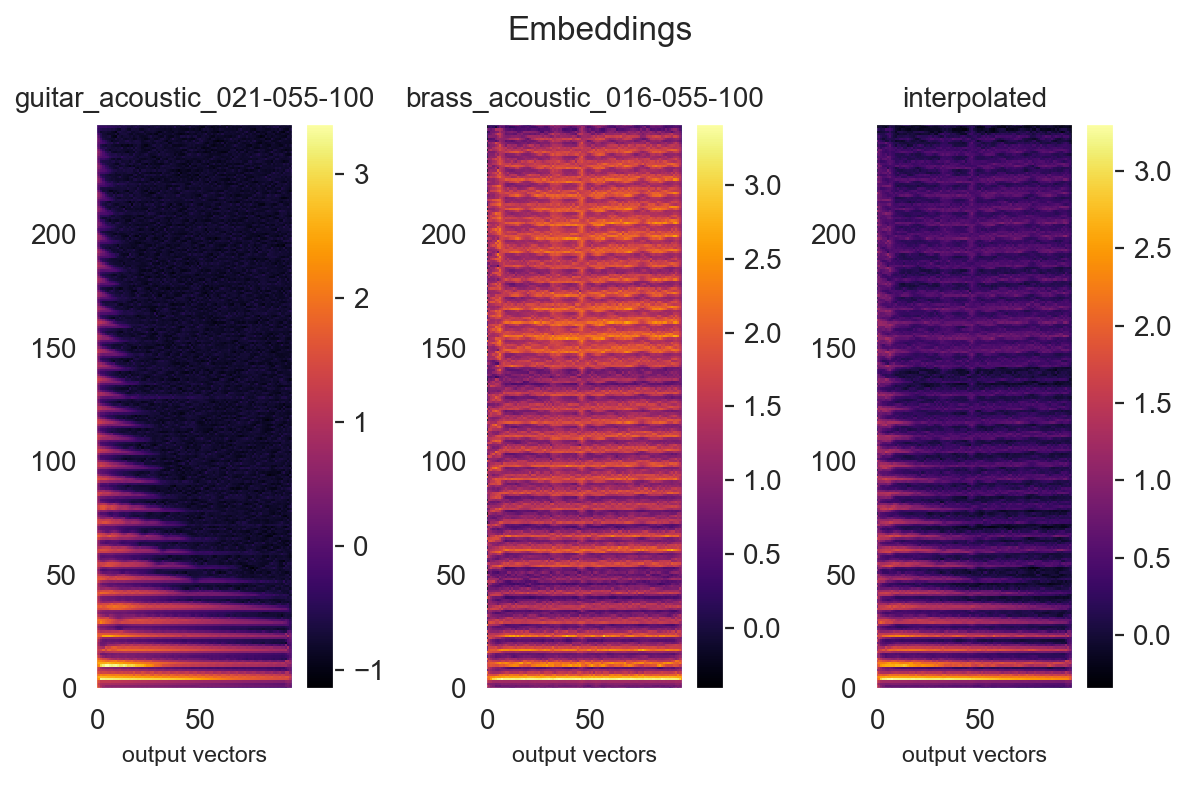
\includegraphics[width=0.60\textwidth]{images/results/single_str/inter_guitar_acoustic_021-055-100&brass_acoustic_016-055-100_original_0.5.png}}\\
        embedding interpolation ~(a)\\
        \makebox{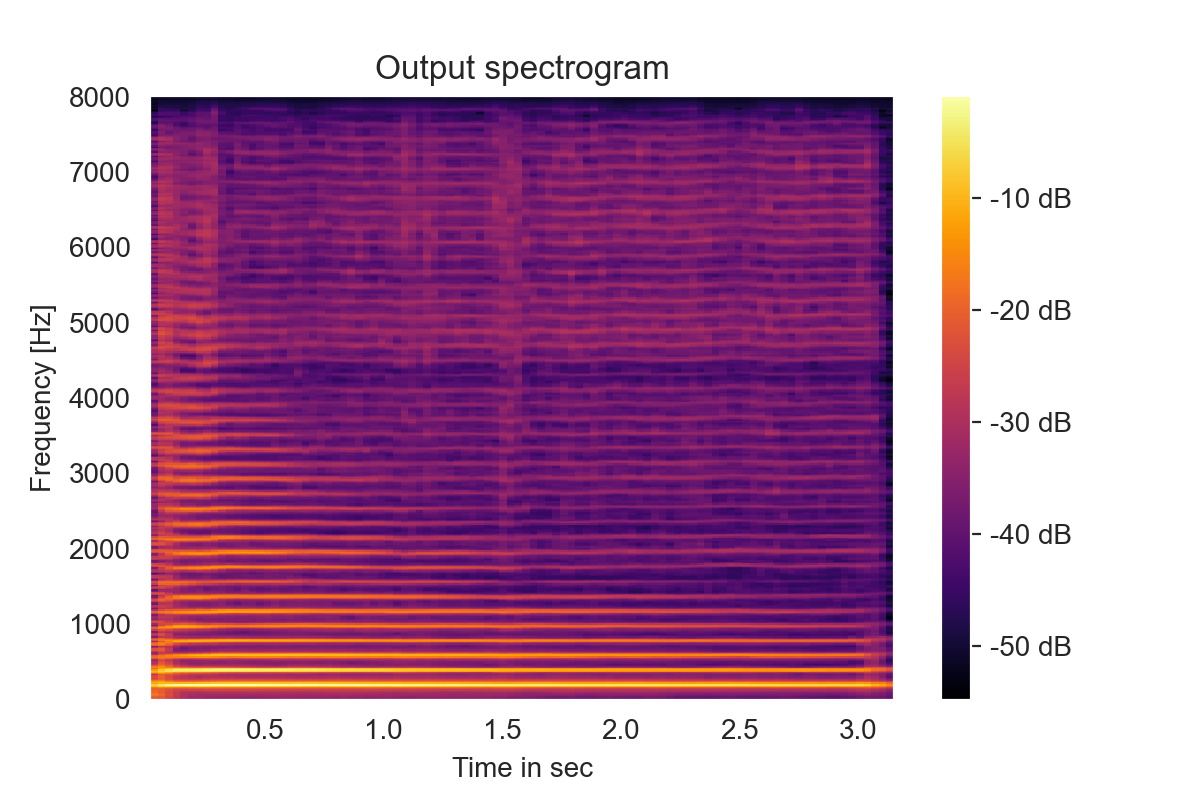
\includegraphics[width=0.60\textwidth]{images/results/single_str/guitar_acoustic_021-055-100&brass_acoustic_016-055-100_output_0.5.png}}\\
        output signal ~(b)
    \end{tabular}}
    \caption{Embeddings of input samples with interpolated embedding and its corresponding output spectrogram - single stride model.}
    \label{fig:res_single_str_2D_inter_output}
\end{figure}

By looking again on the decoded output it can be seen that again both instruments are present. Compared to the result in the first experiments, the guitar sample is more present with these kind of networks. Contrary to the experiment with single sample reconstruction, here the difference between the different strided networks can be noticed even more. With special notice to the higher harmonics of the original brass samples. Those harmonics appear more precise with the single strided network (see figure \ref{fig:res_single_str_2D_inter_output}b). In the output of the double-stride network in figure \ref{fig:res_double_str_2D_inter_output}b the "contours" coming from the brass sample are less sharp then with the single stride.

\begin{figure}[htb!]
    \centering
    \captionsetup{justification=centering}
    \makebox[\textwidth][c]{\begin{tabular}{@{}cc@{}}
        \makebox{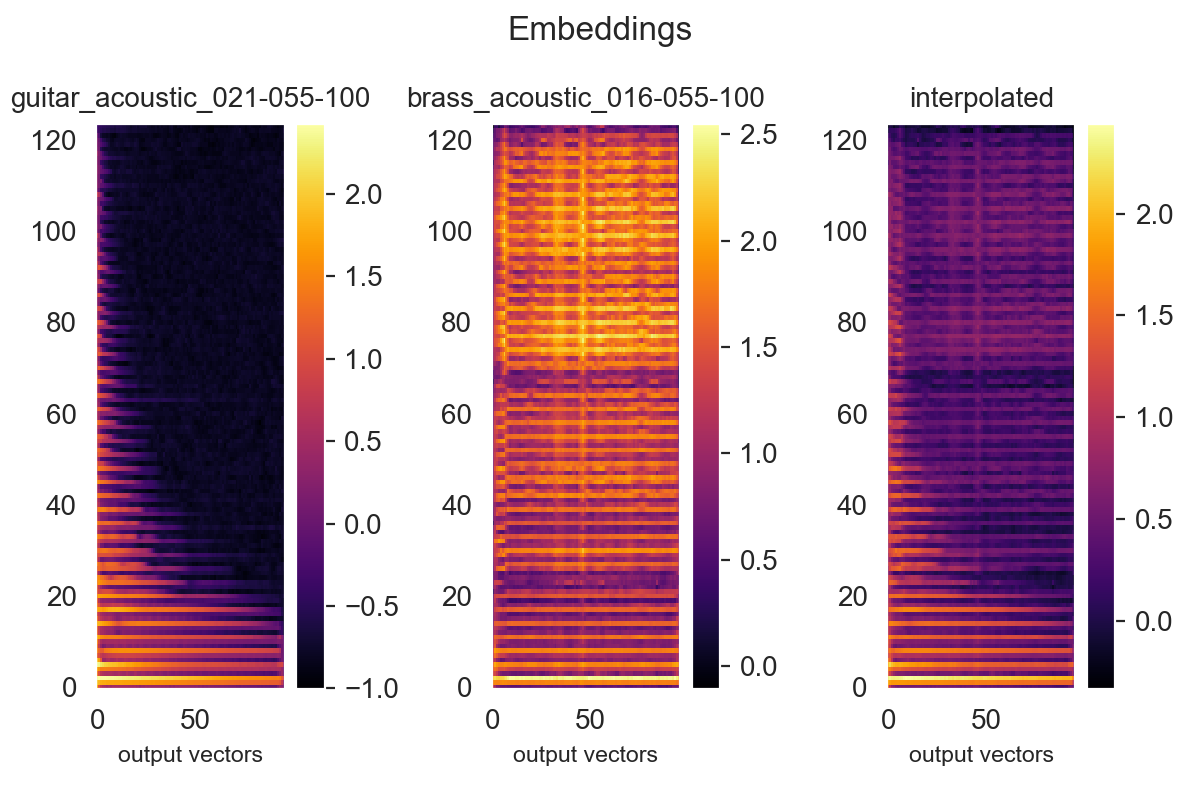
\includegraphics[width=0.60\textwidth]{images/results/double_str/inter_guitar_acoustic_021-055-100&brass_acoustic_016-055-100_original_0.5.png}}\\
        embedding interpolation ~(a)\\
        \makebox{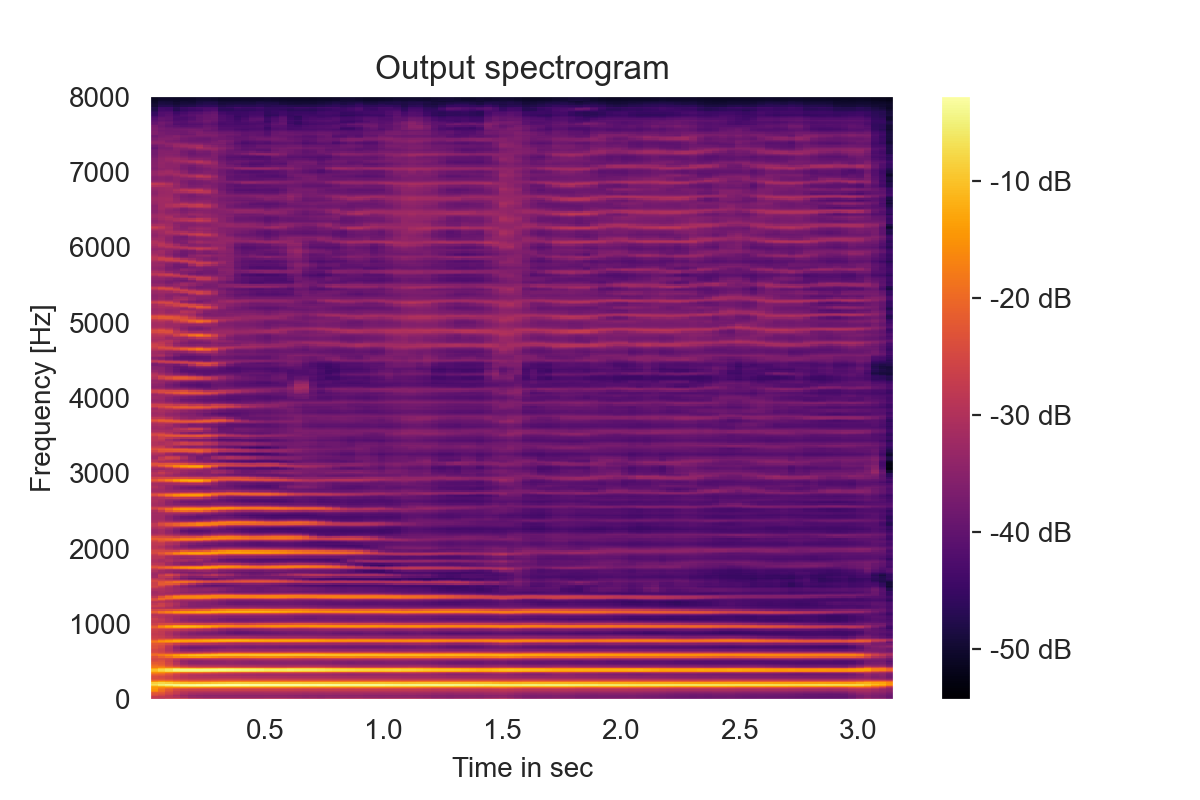
\includegraphics[width=0.60\textwidth]{images/results/double_str/guitar_acoustic_021-055-100&brass_acoustic_016-055-100_output_0.5.png}}\\
        output signal ~(b)
    \end{tabular}}
    \caption{Embeddings of input samples with interpolated embedding and its corresponding output spectrogram - double stride model.}
    \label{fig:res_double_str_2D_inter_output}
\end{figure}

Taking the output of the triple strided network (figure \ref{fig:res_triple_str_2D_inter_output}) into account, the difference to the other networks can be seen clearly. The encoded features again contain the same structure as the input spectrograms, but due to the three-fold striding, just the most significant information is present. Comparing the interpolated embeddings it can also be said that in the latter, the guitar features can be recognized better. Looking at the final output spectrogram in \ref{fig:res_triple_str_2D_inter_output}b it can be seen that the original fine harmonics aren't present anymore. The energy values of the different frequencies over time don't remain constant and show "washed out" contours. Also the fine changes over time are not as precisely present as with previous network configurations. Nevertheless both instrumental features can be recognized in the final output. Again in the discussion part, the auditive quality of all outputs presented here, with and without energy correction, is assessed and brought into relation with the displayed spectrograms here.

\begin{figure}[htb!]
    \centering
    \captionsetup{justification=centering}
    \makebox[\textwidth][c]{\begin{tabular}{@{}cc@{}}
        \makebox{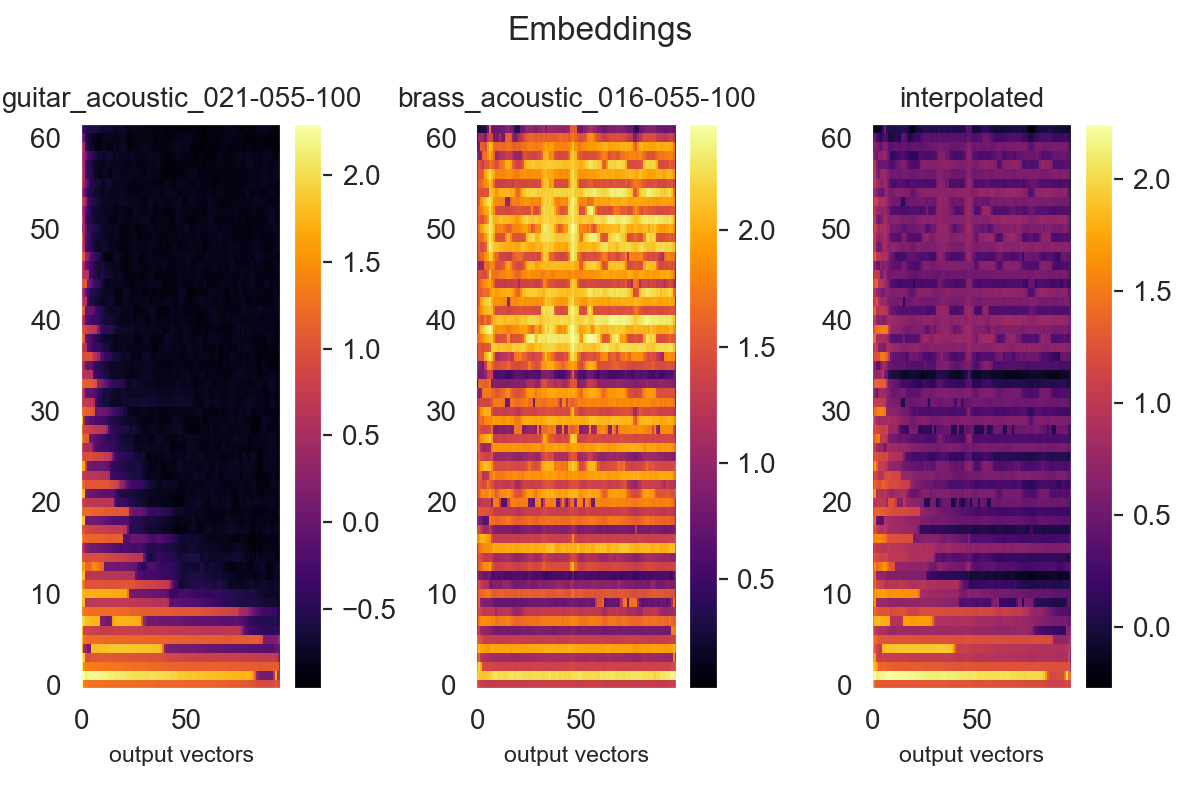
\includegraphics[width=0.60\textwidth]{images/results/triple_str/inter_guitar_acoustic_021-055-100&brass_acoustic_016-055-100_original_0.5.png}}\\
        embedding interpolation ~(a)\\
        \makebox{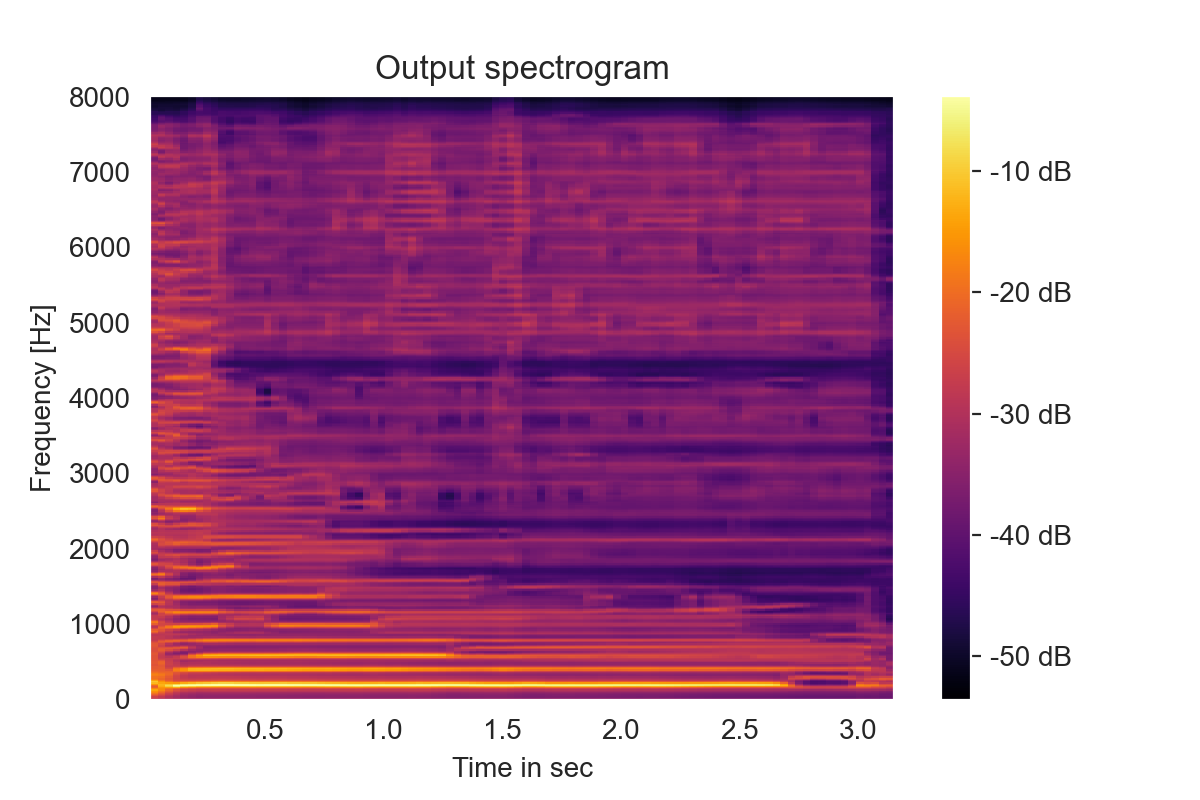
\includegraphics[width=0.60\textwidth]{images/results/triple_str/guitar_acoustic_021-055-100&brass_acoustic_016-055-100_output_0.5.png}}\\
        output signal ~(b)
    \end{tabular}}
    \caption{Embeddings of input samples with interpolated embedding and its corresponding output spectrogram - triple stride model.}
    \label{fig:res_triple_str_2D_inter_output}
\end{figure}



\section{Results with mel-spectrograms}

The final experiments are again done with a 2D convolutional network, but using mel scale spectrograms instead of log-magnitude. In chapter \ref{cha:Experiment} under section \ref{sec:exp_mel} an introduction to the mel-scale has been given. As those log-mel spectrograms are a compressed version of the log-magnitude spectrograms and emphasize the lower frequencies, these experiments are expected to bring different but interesting results. This is again meant regarding the model performance but also towards the quality of reconstructing spectrograms with or without modification of the embeddings. The results again get depicted in tables filled with the MSE scores of training, validation and testing but also the scores regarding specific pitch classes of the test set. Later on again the graphics contain the output spectrograms and embeddings with and without interpolation. Again three different networks with single, double and triple strides were used. Those are similar in their structure to the ones used with log-magnitude spectrograms, which were already explained in the previous chapter.

The following table \ref{tab:res_scores_2D_mel} shows the training, validation and testing scores of all three different networks. First of all the MSE scores of all networks are significantly, higher than the ones of the log-magnitude networks. An exception is the testing score of the single-stride network as it is equal to the training score of the triple-strided log-magnitude network. The scores between the networks also increase with the amount of compression, making the single-stride network again the best performing network regarding its score. Interestingly the validation score of the single-stride network is the only one that is higher as its corresponding training score. The double- and triple-stride networks therefore show that they have a lower score on reconstructing unseen data. Again the auditory quality will be assessed in the next chapter \ref{cha:Discussion}.

\begin{table}[htb!]
    \centering
    \captionsetup{justification=centering}
    \begin{tabular}{|c|c|c|c|}
        \hline
         & \textbf{single-stride} & \textbf{double-stride} & \textbf{triple-stride} \\
         \hline
        \textbf{Training} & 30,579 & 49,685 & 62,833 \\
        \hline
        \textbf{Validation} & 31,084 & 48,439 & 60,471\\
        \hline
        \textbf{Test} & 18,322 & 33,689 & 43,300\\
        \hline
    \end{tabular}
    \caption{MSE-Scores 2D convolutional autoencoder with log-mel spectrograms - single stride, double stride, triple stride.}
    \label{tab:res_scores_2D_mel}
\end{table}

Like in the previous experiments, the network performance has been evaluated towards certain pitch classes. Table \ref{tab:res_scores_2D_pitch_mel} shows the MSE scores of different pitch classes. For comparative reasons, again they got categorized on a scale from 30 to 100 in steps of 5. Contrary to those scores in the previous experiments, here the values show that the lower pitched samples have the best score. With some exceptions/outliers, the error scores increase with a clear trend, the higher pitched the used samples were. Interestingly the difference in the score between the highest and lowest used samples increases the more compression is used. 

\begin{table}[htb!]
\centering
\begin{tabular}{|c|c|c|c|}
\hline
\textbf{pitch} & \textbf{single-stride} & \textbf{double-stride} & \textbf{triple-stride} \\ \hline
\textbf{030}   & 17,178                 & 24,567                 & 30,302                 \\ \hline
\textbf{035}   & 18,380                 & 26,142                 & 36,509                 \\ \hline
\textbf{040}   & 19,382                 & 34,125                 & 44,062                 \\ \hline
\textbf{045}   & 22,036                 & 55,770                 & 51,097                 \\ \hline
\textbf{050}   & 22,398                 & 41,101                 & 49,810                 \\ \hline
\textbf{055}   & 22,159                 & 43,215                 & 56,664                 \\ \hline
\textbf{060}   & 21,472                 & 40,493                 & 54,690                 \\ \hline
\textbf{065}   & 22,303                 & 40,140                 & 51,926                 \\ \hline
\textbf{070}   & 23,875                 & 41,950                 & 50,904                 \\ \hline
\textbf{075}   & 24,571                 & 37,424                 & 49,297                 \\ \hline
\textbf{080}   & 29,053                 & 43,572                 & 60,926                 \\ \hline
\textbf{085}   & 29,395                 & 46,822                 & 62,750                 \\ \hline
\textbf{090}   & 33,316                 & 51,408                 & 72,206                 \\ \hline
\textbf{095}   & 31,385                 & 51,593                 & 70,607                 \\ \hline
\textbf{100}   & 32,129                 & 51,426                 & 70,890                 \\ \hline
\end{tabular}
\caption{MSE-Scores for specific pitch classes using 2D convolutional autoencoder using mel-scale.}
\label{tab:res_scores_2D_pitch_mel}
\end{table}

\subsection{Experiments of single reconstruction}
Similar to the other experiments to assess the ability of reconstructing spectrograms and therefore recreate audio samples, in this section the embeddings and corresponding output spectrograms are depicted. There again the properties and respective differences to the other experiments get assessed. Regarding the auditory quality the results are discussed in chapter \ref{cha:Discussion}. The here shown results again correspond just to the reconstruction of single samples without interpolation. As in these last experiments the mel scale as different scale was used, the corresponding input spectrograms are shown in advance. Figure \ref{fig:res_2D_mel_guit} shows the input spectrogram of the single reconstruction experiments.

\begin{figure}[htb!]
    \centering
    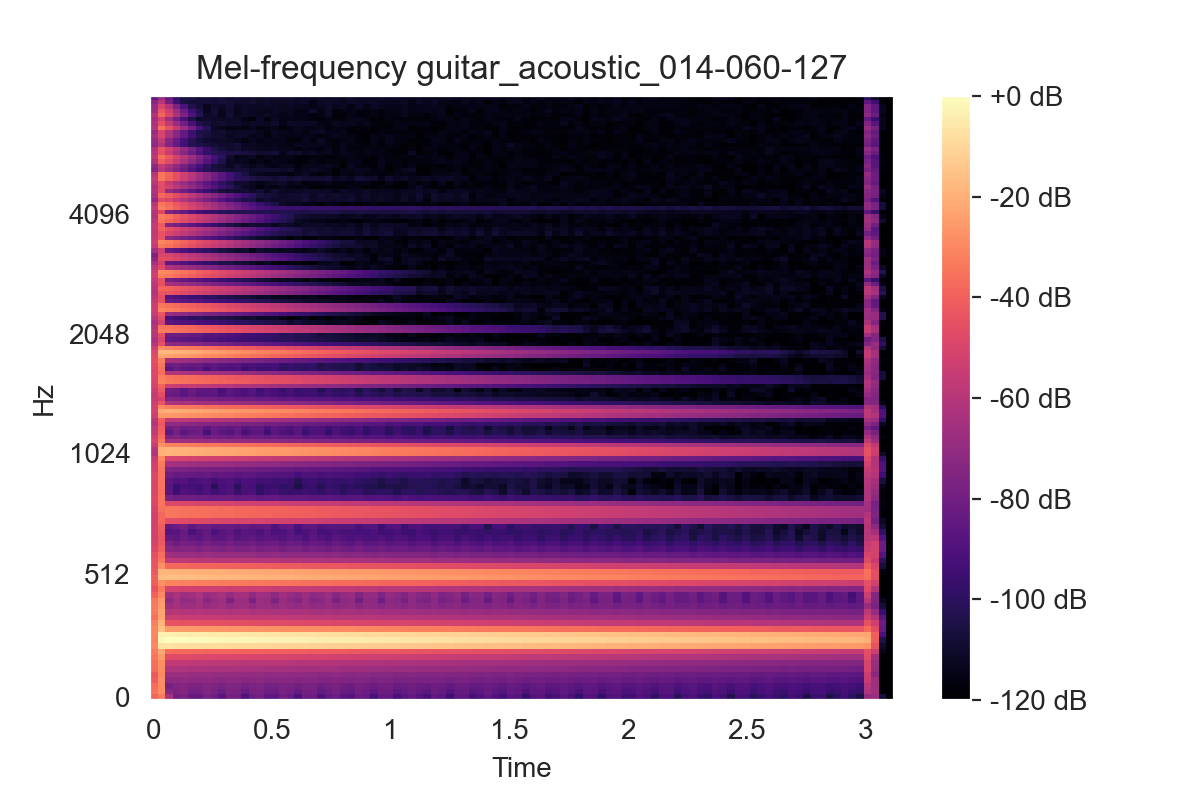
\includegraphics[width=0.60\textwidth]{images/results/mel_guitar_acoustic_014-060-127.png}
    \caption{Original mel-spectrogram of guitar acoustic.}
    \label{fig:res_2D_mel_guit}
\end{figure}

The next three figures (\ref{fig:res_mel_single_str_2D_output_emb}, \ref{fig:res_mel_double_str_2D_output_emb} and \ref{fig:res_mel_triple_str_2D_output_emb}) show the output spectrograms but also the embeddings of the guitar sample depicted in figure \ref{fig:res_2D_mel_guit}. As its known at this point, the mel-spectrograms are already a compressed version log-magnitude spectrograms, as they contain 128 values instead 513. Thus it can be seen on the y-axis of the embeddings, that those embeddings are even more compressed than in the last experiment (size of 56, 28 and 14). Furthermore it can be noticed regarding the embeddings of the first two networks (figures \ref{fig:res_mel_single_str_2D_output_emb}b and \ref{fig:res_mel_double_str_2D_output_emb}b), that contrary to the previous experiments with log-magnitde spectrograms, the low energy areas are positively valued. The high-energy areas and harmonics are therefore negatively valued. Concerning the scale it can be also said that those embeddings have a narrower value range then those in the previous experiments. 

\begin{figure}[htb!]
    \centering
    \captionsetup{justification=centering}
    \makebox[\textwidth][c]{\begin{tabular}{@{}cc@{}}
        \makebox{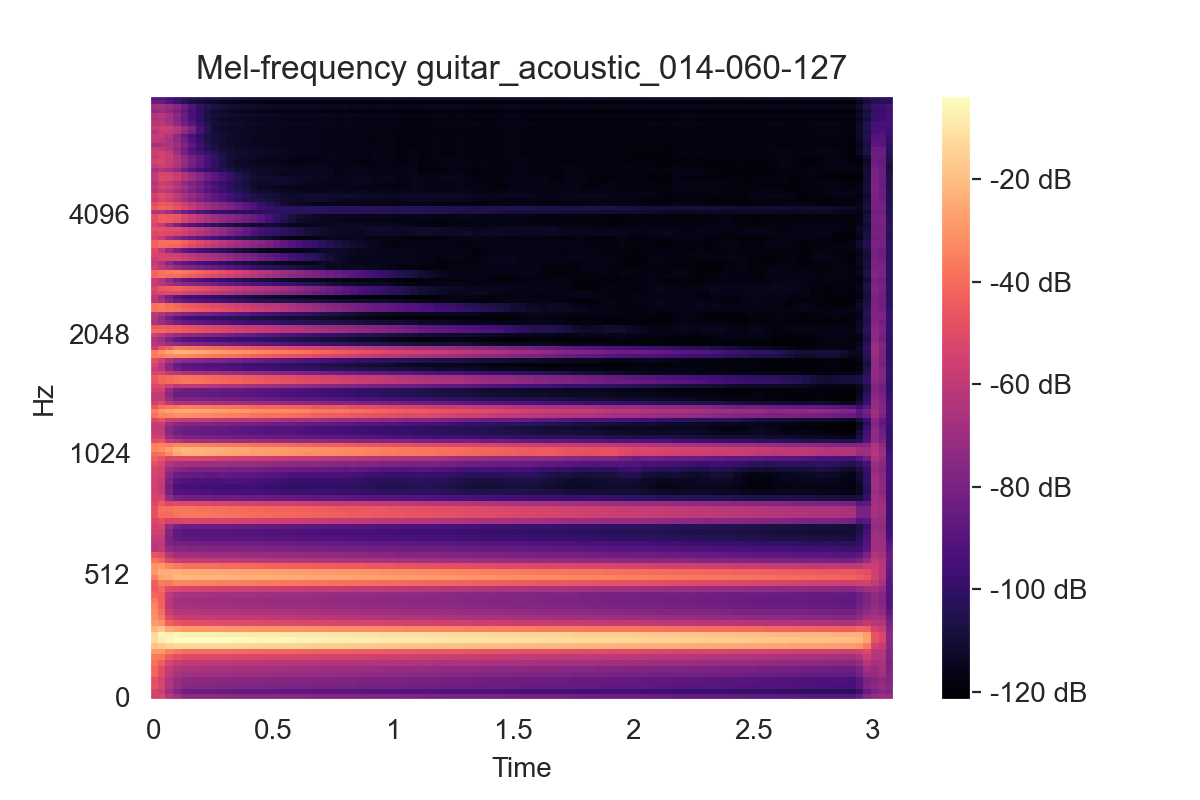
\includegraphics[width=0.5\textwidth]{images/results/mel_single_str/guitar_acoustic_014-060-127.png}}&
        \makebox{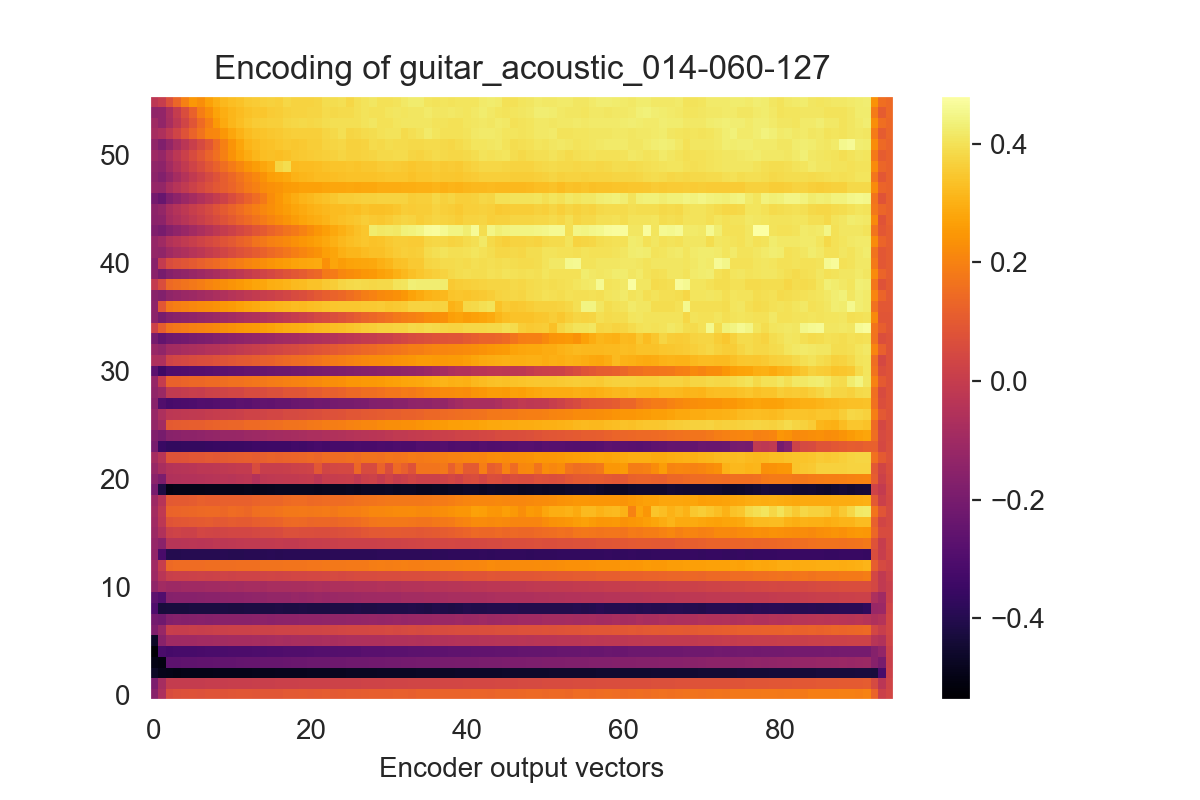
\includegraphics[width=0.5\textwidth]{images/results/mel_single_str/emb_guitar_acoustic_014-060-127.png}}\\
        reconstruction of guitar acoustic ~(a) & embedding of guitar acoustic ~(b)
    \end{tabular}}
    \caption{Reconstructed log-mel spectrogram and corresponding embedding - single-stride network.}
    \label{fig:res_mel_single_str_2D_output_emb}
\end{figure}

In figure \ref{fig:res_mel_single_str_2D_output_emb}a the output of the single strided network can be seen. In comparison to the input spectrogram, its reconstruction is the best out of those three networks, as it contains the most details. Despite of this, it can be seen that the broadband spectra at the beginning and end are not as intense as with the input. Further on it can be seen that changes over time in the frequencies between the lower harmonics are not present in the output. The embeddings in figures \ref{fig:res_mel_single_str_2D_output_emb}b and \ref{fig:res_mel_double_str_2D_output_emb}b show that the features representing the lower harmonics are recognizable as negative values. The latter already shows a lack of features in the higher harmonics. This is caused by the input log-mel spectrograms having a shorter distance between the higher harmonics then in the lower ones. Regarding the output of the double-stride network it can therefore be said that the higher harmonics can be less distinguished from each other then with the single-stride network (see area over >2048 Hz).


\begin{figure}[htb!]
    \centering
    \captionsetup{justification=centering}
    \makebox[\textwidth][c]{\begin{tabular}{@{}cc@{}}
        \makebox{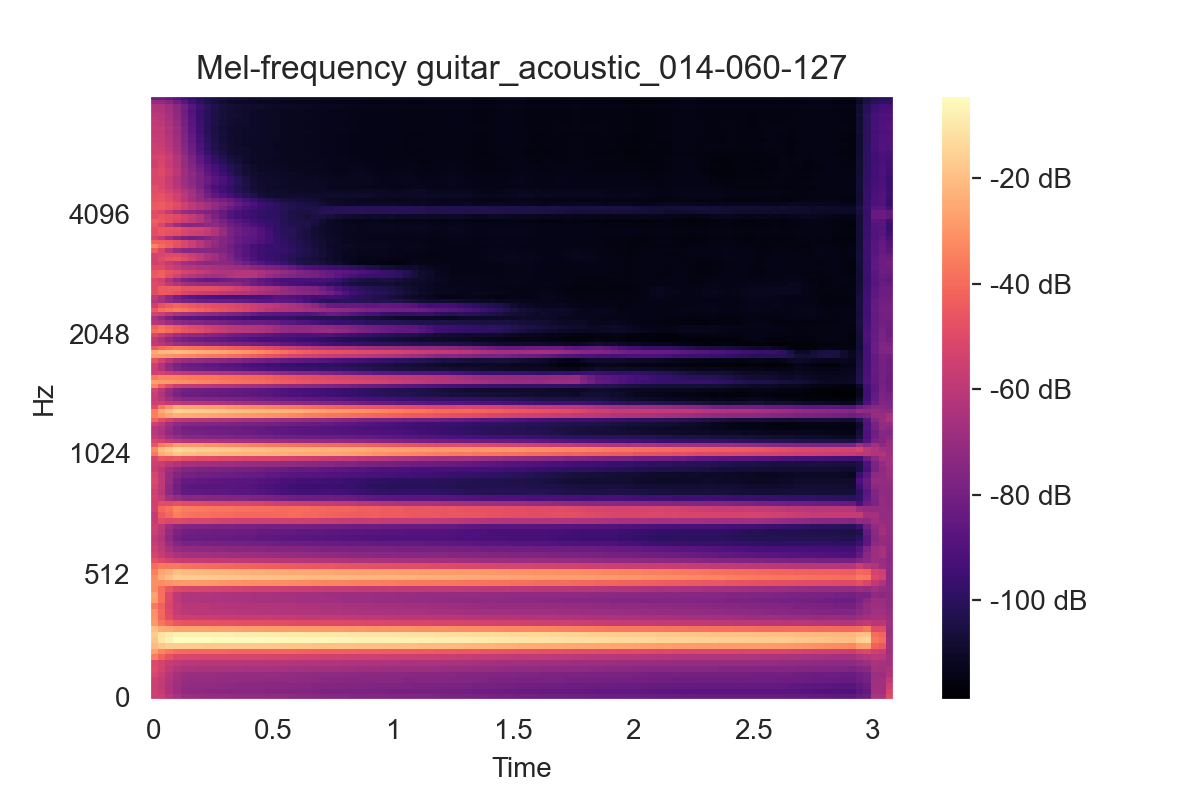
\includegraphics[width=0.50\textwidth]{images/results/mel_double_str/guitar_acoustic_014-060-127.png}}&
        \makebox{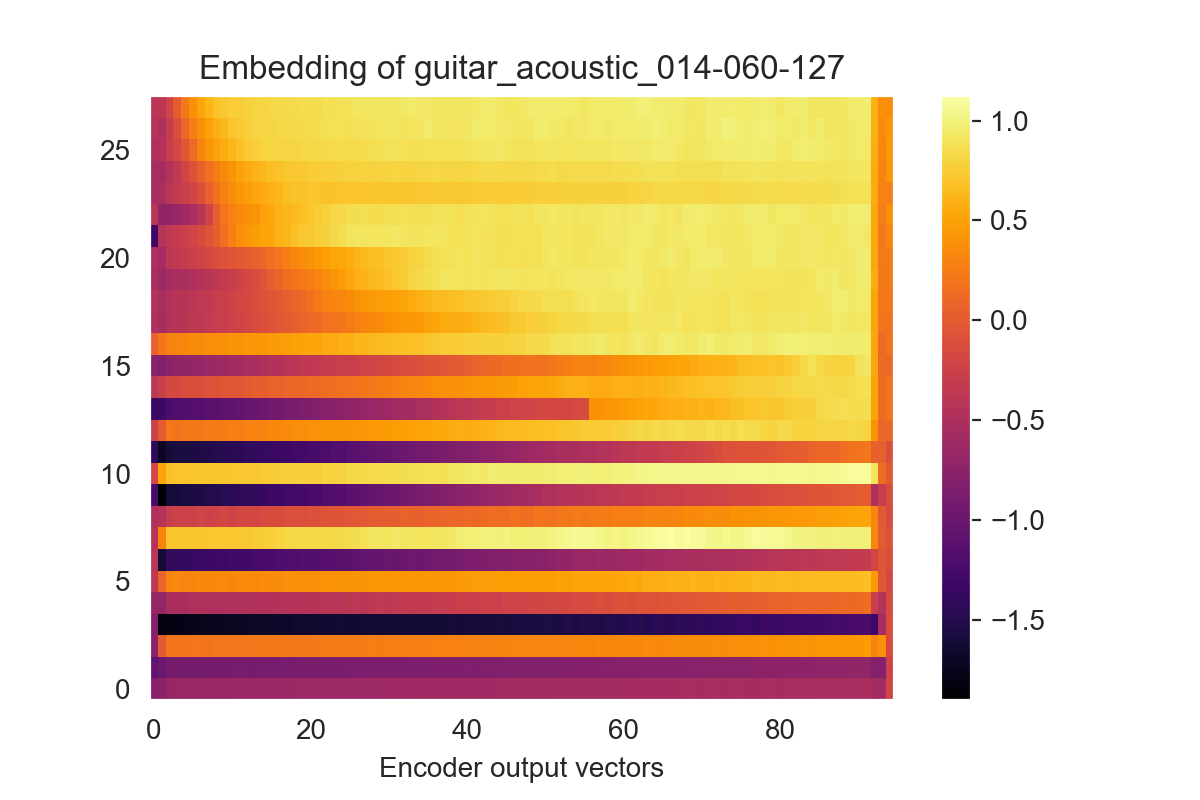
\includegraphics[width=0.5\textwidth]{images/results/mel_double_str/emb_guitar_acoustic_014-060-127.png}}\\
        reconstruction of guitar acoustic ~(a) & embedding of guitar acoustic ~(b)
    \end{tabular}}
    \caption{Reconstructed log-mel spectrogram and corresponding embedding - double-stride network.}
    \label{fig:res_mel_double_str_2D_output_emb}
\end{figure}

Comparing the result of the double-strided network with the one of the triple strided network, significant differences can be discovered. Especially when looking onto the embedding, it can be discovered that due to the small amount of values on the y-axis the features are less distinguishable. Thus it is also more difficult to describe them. Nevertheless it can be said for this input spectrogram, that the colored areas still represent the most significant features that describe the input. Interestingly when looking onto the output spectrogram in \ref{fig:res_mel_triple_str_2D_output_emb}a, regarding the lower harmonics, no differences can be seen to the previous output spectrograms. The part around 4096 Hz also shows some distinct spots that contain more energy, which are not present in the input spectrogram (artefacts).

\begin{figure}[htb!]
    \centering
    \captionsetup{justification=centering}
    \makebox[\textwidth][c]{\begin{tabular}{@{}cc@{}}
        \makebox{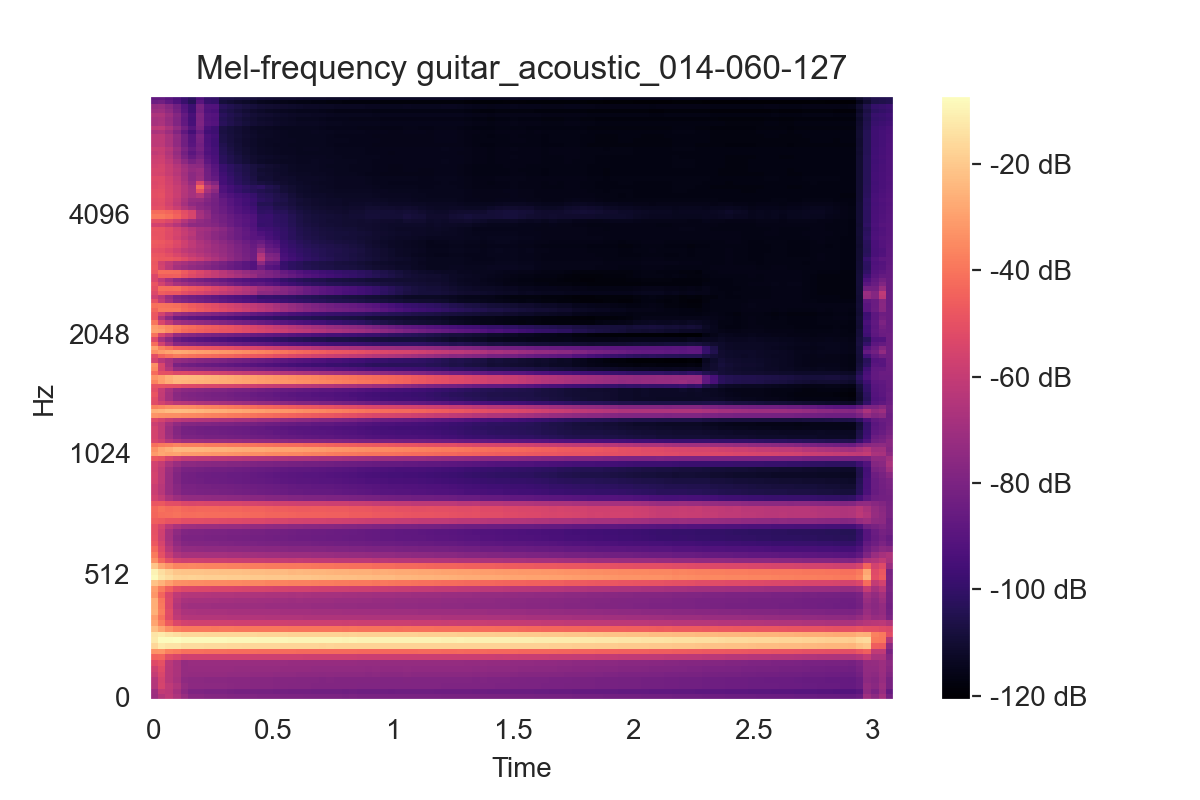
\includegraphics[width=0.5\textwidth]{images/results/mel_triple_str/guitar_acoustic_014-060-127.png}}&
        \makebox{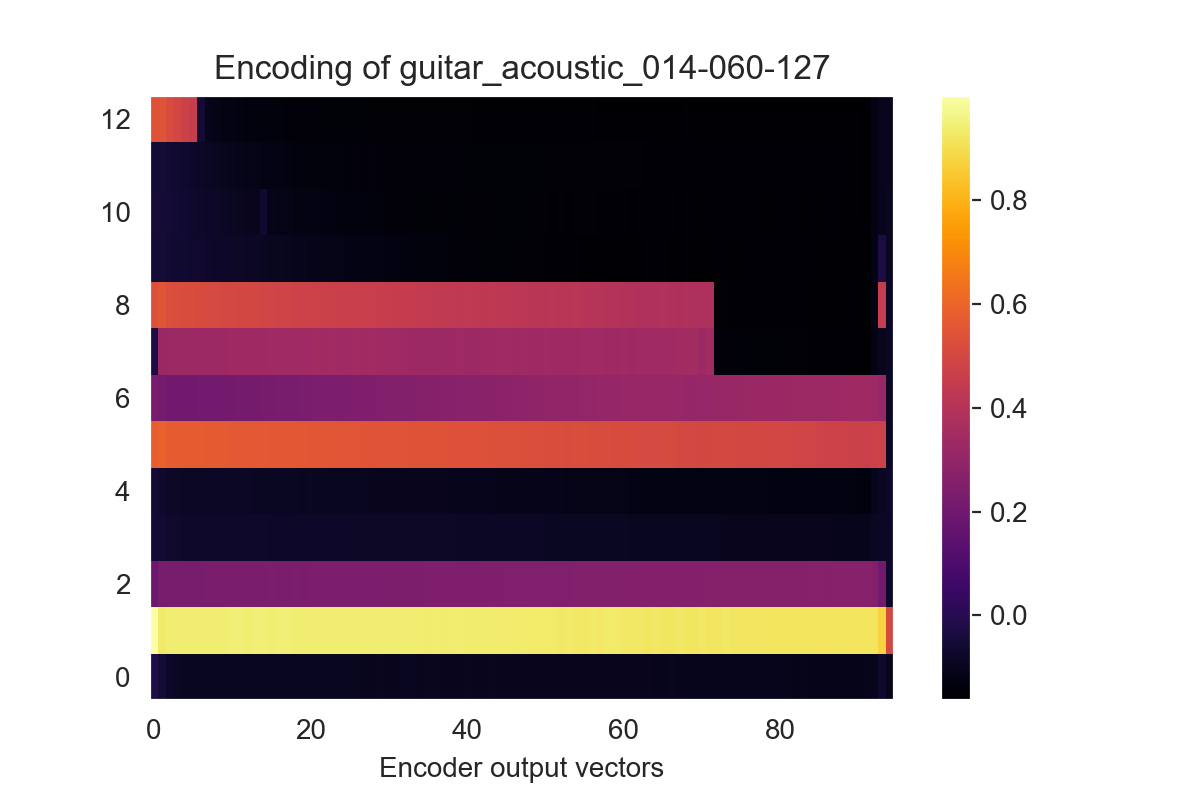
\includegraphics[width=0.5\textwidth]{images/results/mel_triple_str/emb_guitar_acoustic_014-060-127.png}}\\
        reconstruction of guitar acoustic ~(a) & embedding of guitar acoustic ~(b)
    \end{tabular}}
    \caption{Reconstructed log-mel spectrogram and corresponding embedding - triple-stride network.}
    \label{fig:res_mel_triple_str_2D_output_emb}
\end{figure}

\subsection{Experiments with interpolation in embedding}
The final experiments in this work also deal with the introduction of the interpolation step to synthesize novel sounds. With the experiments of reconstructing single audios, it could be seen that despite the small compressed embeddings, the input spectrograms could be reconstructed adequately. Having those smaller embeddings, less values are available to reconstruct spectrograms which in conclusion means that altering those also brings significant changes. This fact makes these experiments even more interesting, as here again, the embeddings of two input samples are interpolated, to generate novel sounds. As an example, the same guitar and brass samples that were used in the previous experiments are utilized to synthesize audio. The following graphics \ref{fig:res_mel_original_guit_brass} show the input log-mel spectrograms of the two source signals. To mention at this point again, the higher harmonics are closer in the scale, while the lower harmonics have a greater distance. Especially when looking at the brass sample this can be noticed as the energy does not fade.

\begin{figure}[htb!]
    \centering
    \captionsetup{justification=centering}
    \makebox[\textwidth][c]{\begin{tabular}{@{}cc@{}}
        \makebox{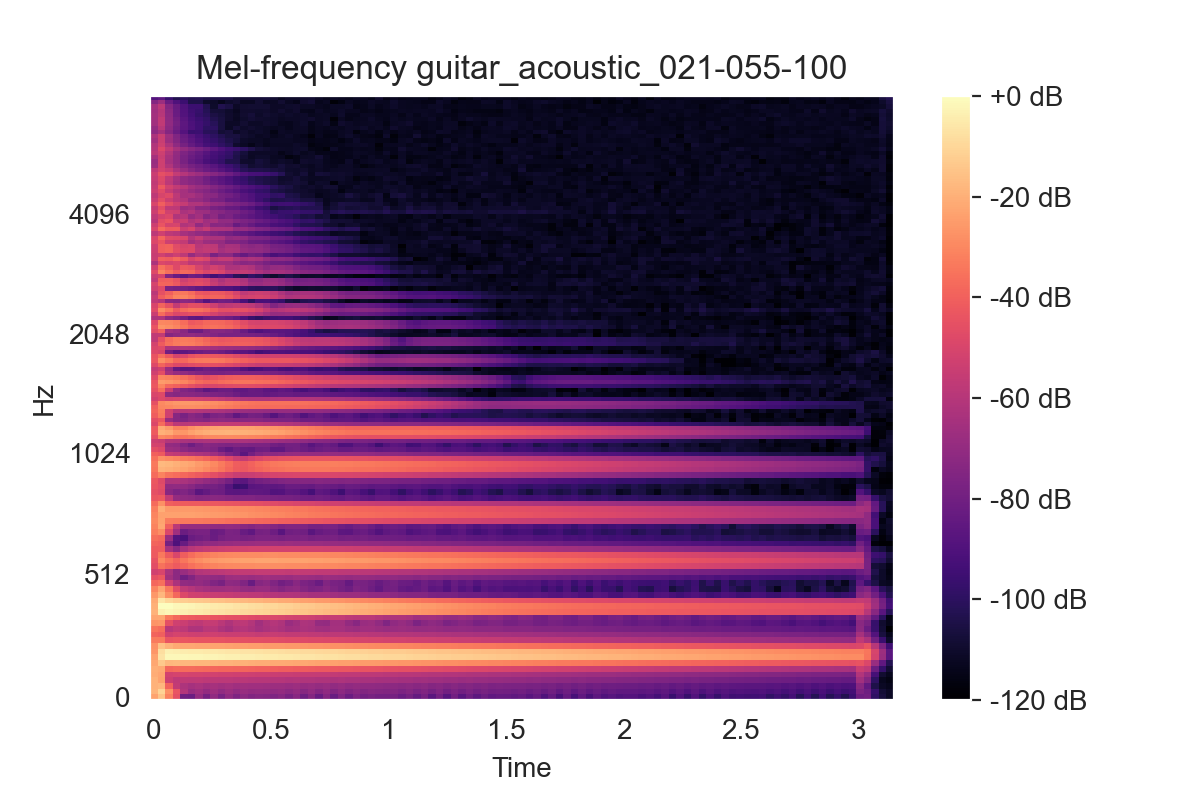
\includegraphics[width=0.5\textwidth]{images/results/mel_guitar_acoustic_021-055-100.png}}&
        \makebox{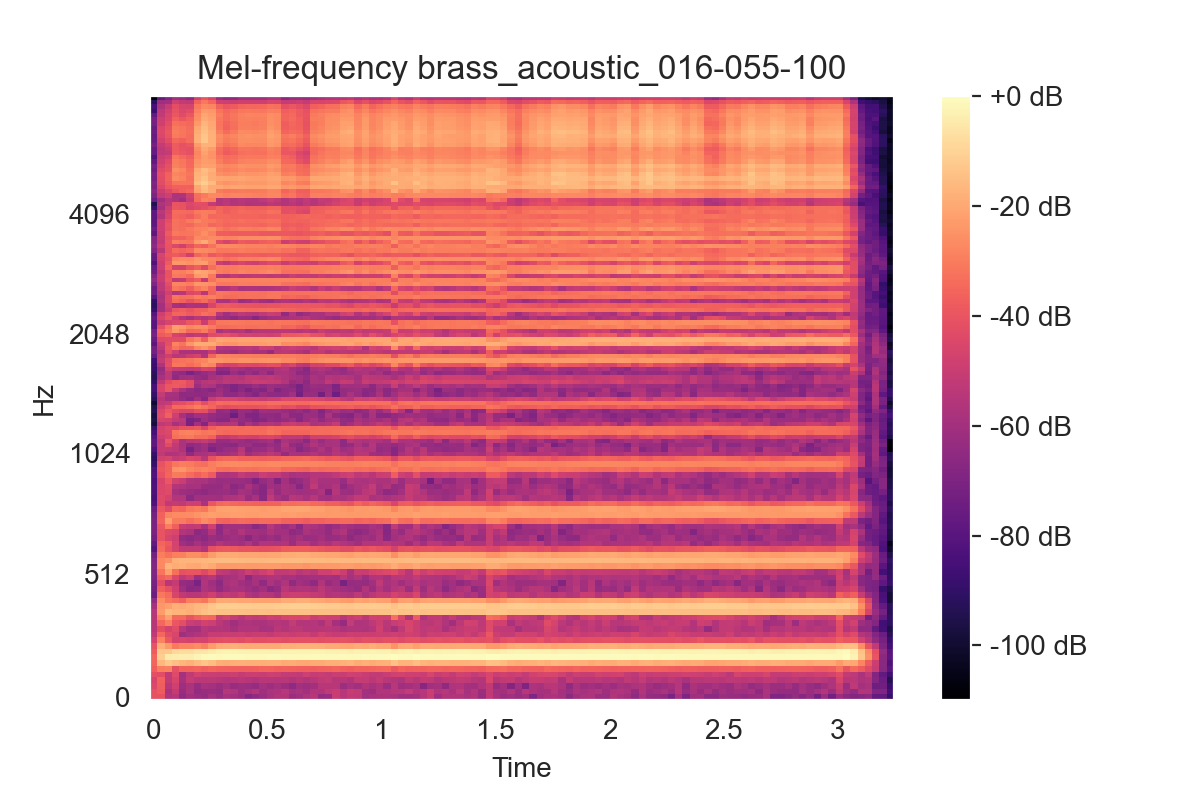
\includegraphics[width=0.5\textwidth]{images/results/mel_brass_acoustic_016-055-100.png}}\\
        original guitar acoustic ~(a) & original brass acoustic ~(b)
    \end{tabular}}
    \caption{Input log-mel spectrograms.}
    \label{fig:res_mel_original_guit_brass}
\end{figure}

Knowing the source log-mel spectrograms, the following graphics show the embeddings of those spectrograms, the interpolated embedding as well as the resulting output spectrogram using again the three differently strided networks (single-, double- and triple-stride). By comparing all the output spectrograms to the two input spectrograms, it again can be said that the output of the single stride network in figure \ref{fig:res_mel_single_str_2D_inter_output}b is the most precise and contains the most characteristics of both instruments. The upper harmonics of the brass sample can still be recognized in the output spectrogram despite the "fading" influence of the guitar sample. Fine changes in the harmonics over time of the trumpet, like at second 1.5, cannot be recognized anymore. Furthermore the guitar sample can also be recognized in the output spectrogram. With a look onto the embeddings those again show the high energy areas with low or negative values. The original low energy areas in turn have positive values. Furthermore due to the little distance between the higher frequency ranges in the input log-mel spectrograms, the embeddings in this area just depict the high-energy areas. This leads the output spectrogram to not have a high precision in the higher harmonics. Nevertheless through interpolation the resulting embedding contains features of both instruments as well as the resulting spectrogram. 

\begin{figure}[htb!]
    \centering
    \captionsetup{justification=centering}
    \makebox[\textwidth][c]{\begin{tabular}{@{}cc@{}}
        \makebox{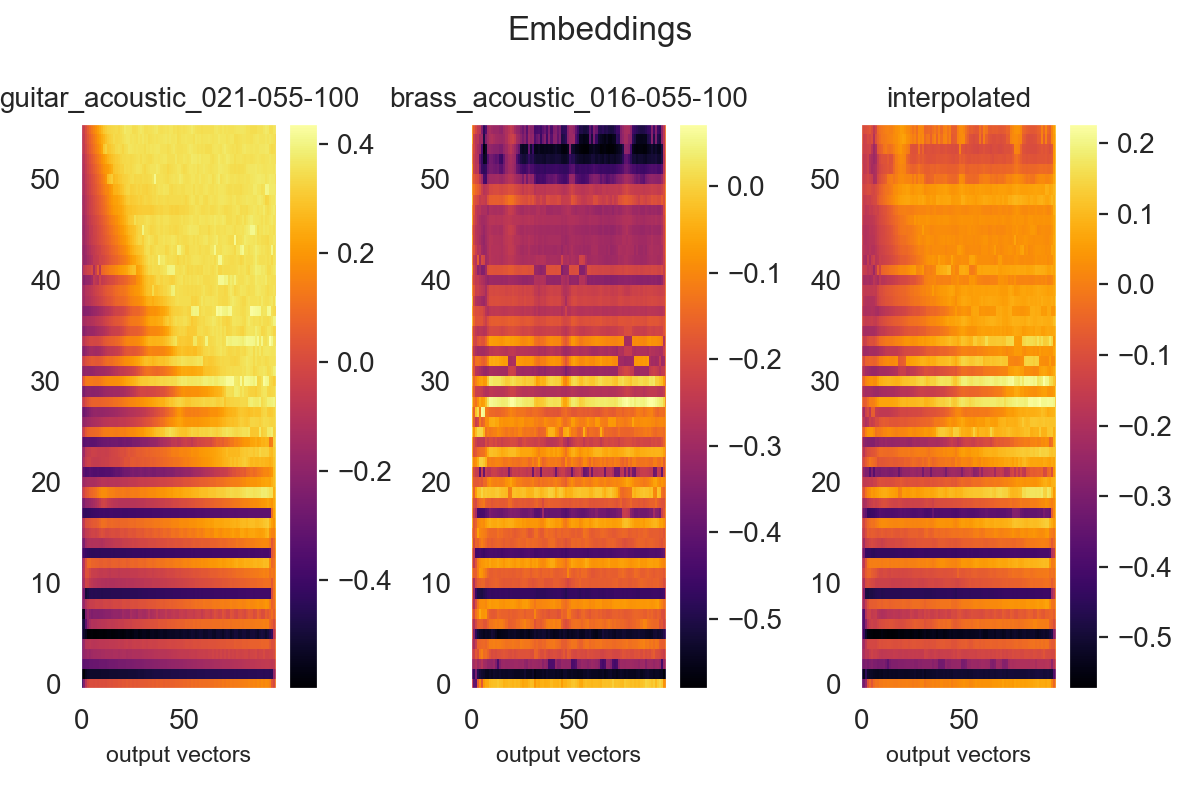
\includegraphics[width=0.60\textwidth]{images/results/mel_single_str/inter_guitar_acoustic_021-055-100&brass_acoustic_016-055-100_original_0.5.png}}\\
        embedding interpolation ~(a)\\
        \makebox{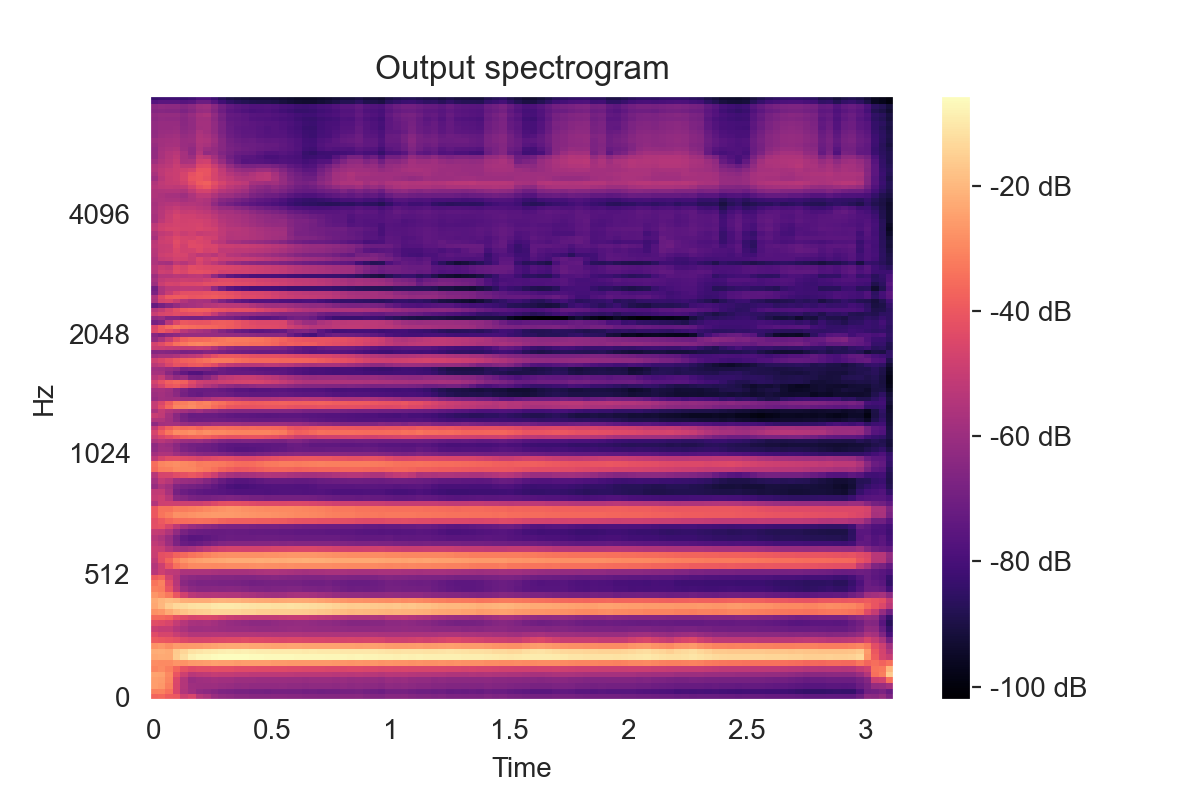
\includegraphics[width=0.6\textwidth]{images/results/mel_single_str/guitar_acoustic_021-055-100&brass_acoustic_016-055-100_output_0.5.png}}\\
        output signal ~(b)
    \end{tabular}}
    \caption{Embeddings of input samples with interpolated embedding and its corresponding output log-mel spectrogram - single-stride network.}
    \label{fig:res_mel_single_str_2D_inter_output}
\end{figure}

Figure \ref{fig:res_mel_double_str_2D_inter_output}, shows the output of the double-stride network where already significant differences to the output of the single-strided network can be seen. First of all regarding the embeddings, the features representing the higher harmonics of both instruments (range >=15) are less intense while the features of the lower harmonics are still distinguishable. Having the interpolated embedding the features of both embeddings can still be recognized, despite the lower precision on the y-axis above 15. As a result in the output spectrogram, the higher harmonics of both instruments are rather "washed out" and appear blurry in the spectrogram. 

\begin{figure}[htb!]
    \centering
    \captionsetup{justification=centering}
    \makebox[\textwidth][c]{\begin{tabular}{@{}cc@{}}
        \makebox{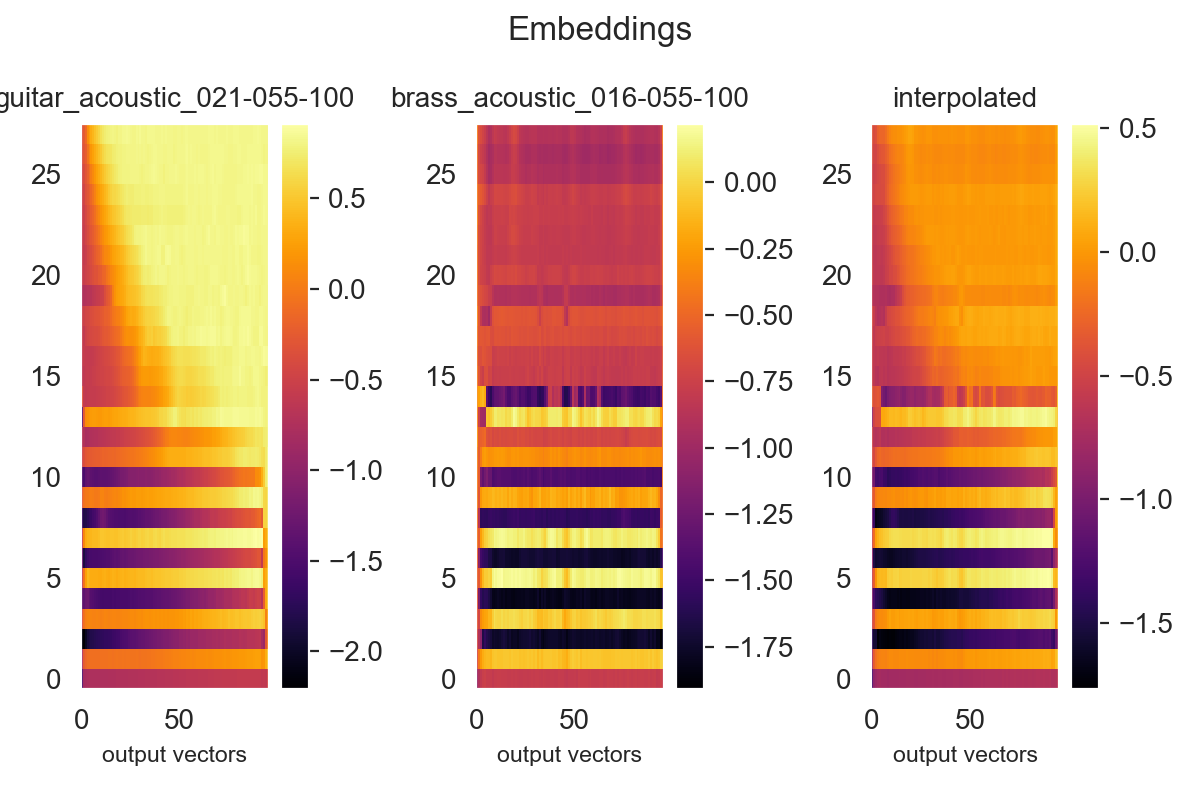
\includegraphics[width=0.6\textwidth]{images/results/mel_double_str/inter_guitar_acoustic_021-055-100&brass_acoustic_016-055-100_original_0.5.png}}\\
        embedding interpolation ~(a)\\
        \makebox{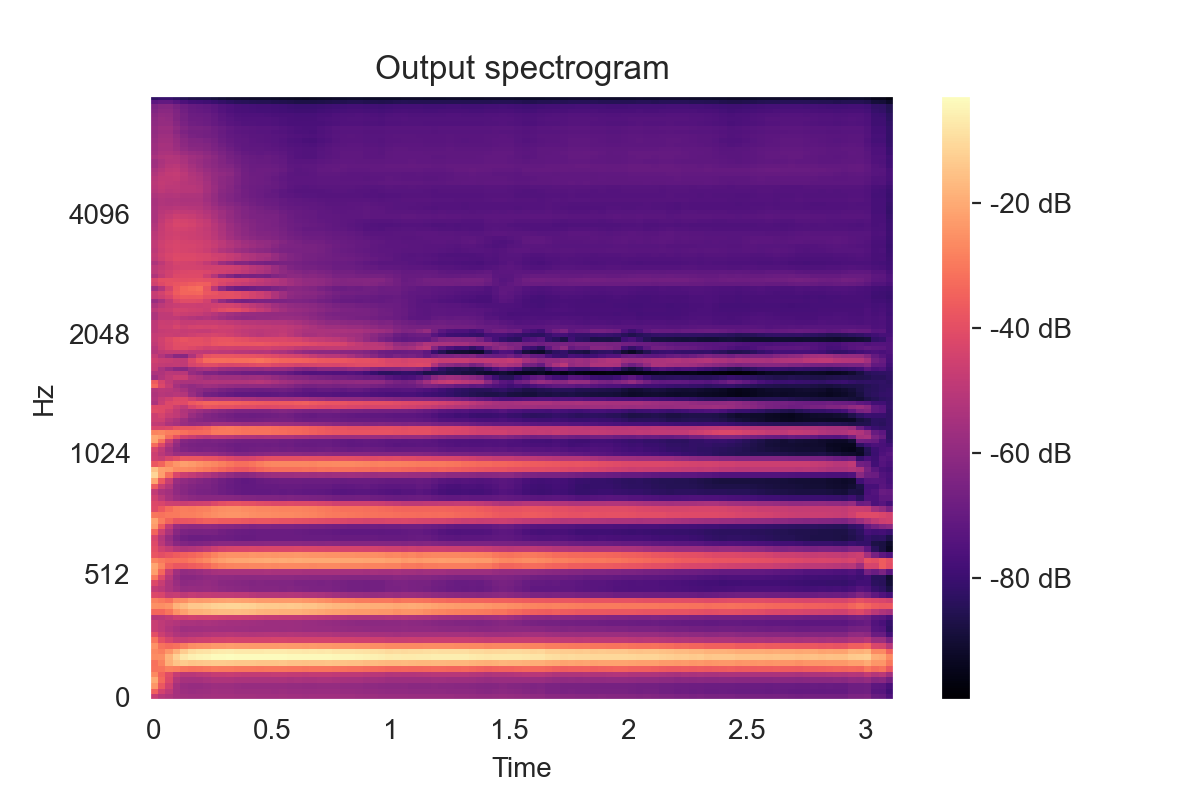
\includegraphics[width=0.6\textwidth]{images/results/mel_double_str/guitar_acoustic_021-055-100&brass_acoustic_016-055-100_output_0.5.png}}\\
        output signal ~(b)
    \end{tabular}}
    \caption{Embeddings of input samples with interpolated embedding and its corresponding output log-mel spectrogram - double-stride network.}
    \label{fig:res_mel_double_str_2D_inter_output}
\end{figure}

Coming to the output of the triple-stride network in figure \ref{fig:res_mel_triple_str_2D_inter_output}, here it can be seen that the features contained in the embeddings have no common structure with the input spectrograms. The values therefore cannot be described sufficiently. Also those appear different to the one depicted in figure \ref{fig:res_mel_triple_str_2D_output_emb}b. When looking at the output spectrogram generated of the interpolated embedding, it can be seen that in the area around 1024 to 2048 significant energy changes regarding certain frequencies are present which cannot be recognized in the input. Similar to the output of the previous network in figure \ref{fig:res_mel_double_str_2D_inter_output}b fine structures of the input are also not present anymore. 

\begin{figure}[htb!]
    \centering
    \captionsetup{justification=centering}
    \makebox[\textwidth][c]{\begin{tabular}{@{}cc@{}}
        \makebox{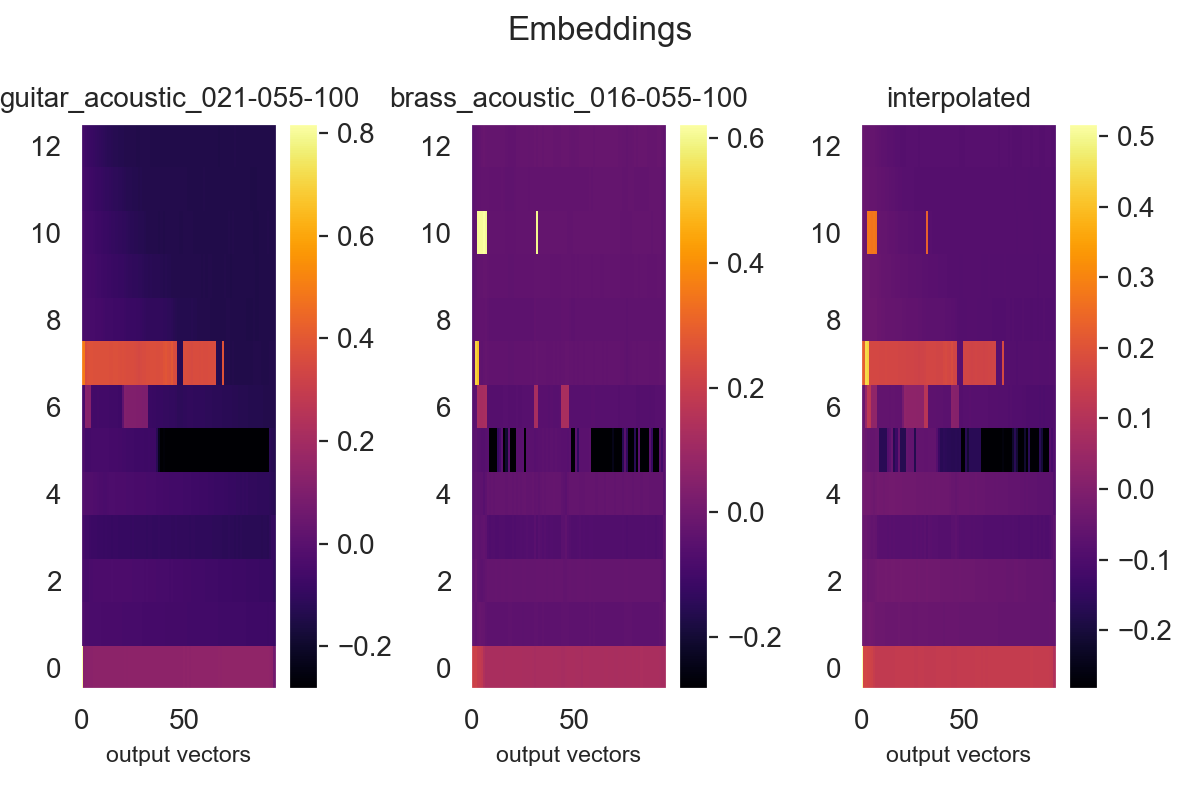
\includegraphics[width=0.6\textwidth]{images/results/mel_triple_str/inter_guitar_acoustic_021-055-100&brass_acoustic_016-055-100_original_0.5.png}}\\
        embedding interpolation ~(a)\\
        \makebox{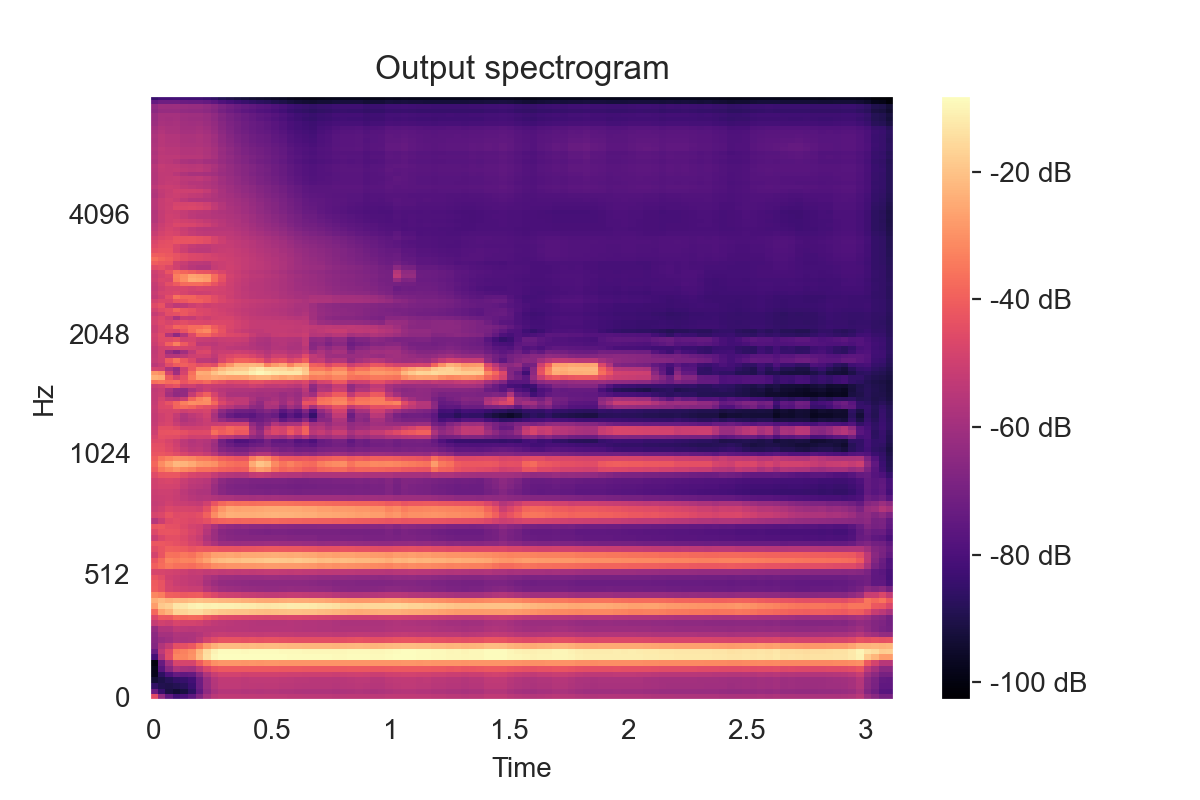
\includegraphics[width=0.6\textwidth]{images/results/mel_triple_str/guitar_acoustic_021-055-100&brass_acoustic_016-055-100_output_0.5.png}}\\
        output signal ~(b)
    \end{tabular}}
    \caption{Embeddings of input samples with interpolated embedding and its corresponding output log-mel spectrogram - triple-stride network.}
    \label{fig:res_mel_triple_str_2D_inter_output}
\end{figure}